\documentclass[11pt]{amsart}
\usepackage[margin=1in]{geometry}
\usepackage{amssymb,amsmath,mathtools}
\usepackage{booktabs}
\usepackage{array}
\usepackage{xcolor}
\usepackage{graphicx}
\usepackage{url}
\usepackage[colorlinks=true,linkcolor=blue!50!black,citecolor=blue!50!black,urlcolor=blue!50!black]{hyperref}

% ------------------------------------------------------------------ macros
\newcommand{\R}{\mathbb{R}}
\newcommand{\C}{\mathbb{C}}
\newcommand{\E}{\mathcal{E}}
\newcommand{\Hs}{\mathbb{H}}
\newcommand{\LD}{L_\Delta}
\newcommand{\eps}{\varepsilon}
\newcommand{\one}{\mathbf{1}}
\newcommand{\dd}{\,\mathrm{d}}
\newcommand{\e}[1]{\cdot 10^{#1}}
\DeclareMathOperator{\Ein}{Ein}
\DeclareMathOperator{\Cin}{Cin}
\DeclareMathOperator{\Ci}{Ci}
\DeclareMathOperator{\re}{Re}
\DeclareMathOperator{\im}{Im}
\DeclareMathOperator{\dist}{dist}

\newtheorem{theorem}{Theorem}[section]
\newtheorem{proposition}[theorem]{Proposition}
\newtheorem{lemma}[theorem]{Lemma}
\newtheorem{corollary}[theorem]{Corollary}
\theoremstyle{definition}
\newtheorem{definition}[theorem]{Definition}
\newtheorem{conjecture}[theorem]{Conjecture}
\theoremstyle{remark}
\newtheorem{remark}[theorem]{Remark}

\numberwithin{equation}{section}
\emergencystretch=3em

\begin{document}

\title[A boundary trace identity for the logarithmic Laplacian]{A boundary trace identity for the logarithmic Laplacian on an interval, and simplicity of its Dirichlet spectrum}

\author{Johann Alexander Botha}
\address{GenusCore}
\email{info@genuscore.com}

\date{Draft of 31 October 2026}

\subjclass[2020]{35R11 (primary); 35P15, 47A75, 47G30, 60G51 (secondary)}
\keywords{logarithmic Laplacian, Dirichlet eigenvalues, boundary trace, Pohozaev identity, simple eigenvalues, Hadamard formula, Wiener--Hopf factorisation, complete Bernstein function}

\begin{abstract}
Let $\LD$ be the logarithmic Laplacian, the operator with Fourier symbol $2\log|\xi|$, on a bounded interval $I$ with Dirichlet exterior condition. We prove that every eigenfunction $u$ has a logarithmic boundary trace: writing $\ell(x)=\log(1/\dist(x,\partial I))$, at each endpoint the limit $A_\pm(u)$ of $u(x)\,\ell(x)^{1/2}$ exists, and $u(x)=A_\pm(u)\,\ell(x)^{-1/2}+O(\ell(x)^{-1})$ with an explicit constant. We then prove the trace identity $A_+(u)^2=A_-(u)^2=\|u\|_{L^2}^2/|I|$ from an exact identity that compares an eigenfunction with its dilation about one endpoint. As in Kwa\'snicki's short proof for the fractional Laplacian, the identity implies that every Dirichlet eigenvalue of $\LD$ on an interval is simple, so every eigenfunction is even or odd. The proofs combine the Wiener--Hopf factorisation of the variance-gamma symbol on a half-line with the fact that the interaction kernel of $\LD$ between disjoint sets is exactly $|x-y|^{-1}$. Uncertified finite-element computations illustrate the results. Existence of the trace, the trace identity and simplicity were obtained earlier in an unrefereed manuscript posted on 27 October 2026 on rStation, a platform for AI research agents; existence of the trace had been derived, and a remainder of the same order stated, in public research notes on the localized Weil operator; and a preprint since withdrawn by its authors announced, with a proof that was withdrawn and without establishing that the trace exists, a Pohozaev identity that formally contains the trace identity. What differs here is a self-contained proof, along essentially the same Wiener--Hopf route as the rStation manuscript, of the remainder bound with an explicit constant, and a different, Pohozaev-type proof of the trace identity and of simplicity; the one-endpoint dilation identity and an identity for even--odd pairs of eigenfunctions are, to our knowledge, new.
\end{abstract}

\maketitle


% =====================================================================
\section{Introduction}\label{sec:intro}

\subsection{Background and open questions}\label{sec:background}
The logarithmic Laplacian $\LD=\frac{d}{ds}\big|_{s=0}(-\Delta)^s$ is the singular integral operator with Fourier symbol $2\log|\xi|$ \cite[Thm.~1.1]{CW19}. Chen and Weth~\cite{CW19} set up its Dirichlet problem on bounded domains (see also~\cite{JSW20}). They proved that the Dirichlet eigenvalues form a sequence $\mu_1<\mu_2\le\mu_3\le\cdots\to\infty$ with $\mu_1$ simple and with a positive eigenfunction \cite[Thm.~1.4]{CW19}, and that solutions decay like $O(\ell(\dist(x,\partial\Omega))^{-\tau})$ for every $\tau<\frac12$ \cite[Thm.~1.11]{CW19}, where
\[
\ell(r):=\log\tfrac1r,\qquad 0<r<1 .
\]
Scaling, Weyl asymptotics and eigenvalue bounds are in~\cite{LW21,CV23}. Feulefack, Jarohs and Weth~\cite{FJW22} showed that $\LD$ governs the small-order asymptotics $\lambda_{k,s}=1+s\mu_k+o(s)$ of the fractional Dirichlet eigenvalues, and that eigenfunctions of $\LD$ are bounded and continuous \cite[Cor.~1.4]{FJW22}. Hern\'andez-Santamar\'ia, L\'opez R\'ios and Salda\~na proved the sharp bound $|u|\le C\ell(\dist(x,\partial\Omega))^{-1/2}$ for bounded weak solutions with bounded right-hand side \cite[Thm.~1.1]{HLS25}, showed that it is optimal \cite[Thm.~1.2]{HLS25}, and proved a Hopf-type lemma, $\liminf u\,\ell^{1/2}>0$, for nonnegative supersolutions \cite[Thm.~1.4]{HLS25}. (Their $\ell(r)=1/|\ln\min(r,0.1)|$ is essentially the reciprocal of ours.) Pollastro and Soave proved Hopf lemmas for $\LD u\ge Vu$ with bounded $V$, including an antisymmetric one \cite[Lemmas~3.4, 3.11]{PS25}. Finite elements and numerical eigenvalues on $(-1,1)$ are in~\cite{HJSS25}, and interior regularity and extension results in~\cite{ClS24,JKW26,CHW23}. The \emph{regional} logarithmic Dirichlet Laplacian of~\cite{GM25,RoSt26}, whose eigenfunctions on an interval are Legendre polynomials, is a different operator.

For eigenfunctions on an interval, the literature in journals and on arXiv left three questions open. Statements and proofs addressing them have been posted in recent unrefereed work, discussed in Section~\ref{sec:novelty}; for question~(2), that work, like this paper, covers only the one-dimensional eigenfunction case of the identity of~\cite{AGV24}.
\begin{enumerate}
\item \emph{Boundary limit.} For general eigenfunctions this literature gives the upper bound $|u|\le C\ell(\dist(x,\partial I))^{-1/2}$ \cite[Thm.~1.1]{HLS25} and, for nonnegative supersolutions, the Hopf-type lower bound $\liminf u\,\ell^{1/2}>0$ \cite[Thm.~1.4]{HLS25}. The latter applies directly to the first eigenfunction $u_1$ when $\mu_1(I)\ge0$, and, combined with the scaling law (Lemma~\ref{lem:dilation}), on every interval, as an external reviewer pointed out to us: for $0<\theta\le e^{\mu_1(I)/2}$, $u_1(\cdot/\theta)$ is a positive first eigenfunction on $\theta I$ with eigenvalue $\mu_1(I)-2\log\theta\ge0$; distances to the boundary scale by $\theta$, and $\ell(\theta d)=\ell(d)+\log\frac1\theta$, so that $\ell(\theta d)/\ell(d)\to1$ as $d\downarrow0$; hence $\liminf u_1(x)\,\ell(\dist(x,\partial I))^{1/2}>0$ at both endpoints of every interval. This also follows directly from the Hopf lemma with bounded potential \cite[Lemma~3.11]{PS25}, applied with $V\equiv\mu_1(I)$ on a short interval at the endpoint. The eigenfunction of the lowest odd eigenvalue is of one sign on each half of $I$, and the antisymmetric Hopf lemma \cite[Lemma~3.4]{PS25} gives the same lower bound for it (see after the proof of Theorem~\ref{thm:C}). These bounds do not give the existence of $\lim u\,\ell(\dist(x,\partial I))^{1/2}$, and for the other sign-changing eigenfunctions no lower bound follows from Hopf-type lemmas. That limit was derived for eigenstates of the localized Weil operator in the research notes \cite[PL-319--PL-323]{Mathia26}, which also state a remainder $O(\ell^{-1})$ \cite[PL-329, PL-336, PL-337]{Mathia26}, and proved in the manuscript \cite[\S3.3]{BT26}. (For the family of fractional eigenfunctions, the optimal boundary rate uniform in $s$ is open \cite[Rem.~1.2(iii)]{FJW22}.)
\item \emph{Pohozaev identity.} Write $\delta_\Omega=\dist(\cdot,\partial\Omega)$. A Pohozaev identity for $\LD$ with boundary term $u^2\ln(\delta_\Omega^{-2})\,(x\cdot\nu)$ was stated in \cite[Thm.~2.3]{AGV24} under the assumption that this boundary trace exists, and in \cite[Cor.~3.8]{AGV24} for all bounded weak solutions on $C^{1,1}$ domains, without a proof that the trace exists. The preprint was withdrawn by its authors (arXiv v2, 26 April 2025) ``due to a crucial error in Proof of Pohozaev identity''. A later paper of the same authors does not use a Pohozaev identity and leaves the corresponding non-existence question open \cite[\S6]{AGV25}. A whole-space identity without boundary term is \cite[Prop.~6.1]{CZ25}. In one dimension and for eigenfunctions, the announced identity, applied on translates of $I$, formally gives each endpoint identity $\int_Iu^2=|I|A_\pm(u)^2$ separately (Remark~\ref{rem:AGV}), and these identities follow from \cite[Cor.~2.3]{BT26}.
\item \emph{Simplicity.} In this literature only $\mu_1$ was known to be simple; \cite{CW19,HJSS25} write $\mu_1<\mu_2\le\cdots$, and the same holds in recent work on the Fu\v{c}\'ik spectrum~\cite{AM26} and on indefinite weights~\cite{AMV26}. Simplicity of every eigenvalue on an interval is proved in \cite[Cor.~2.3]{BT26}.
\end{enumerate}

\subsection{Related results}
For $(-\Delta)^s$ the Pohozaev identity of Ros-Oton and Serra \cite[Thm.~1.1]{RS14} has the boundary term $\Gamma(1+s)^2(u/\delta_\Omega^s)^2$. Simplicity of all Dirichlet eigenvalues of $(-\Delta)^s$ on an interval was proved by Fall, Ghimenti, Micheletti and Pistoia \cite[Cor.~2]{FGMP23}; earlier results covered $s=\frac12$~\cite{KKMS10} and $s\ge\frac12$~\cite{Kw12}. Kwa\'snicki~\cite{Kw23} gave a one-paragraph proof (see also \cite[\S4.1]{DFW24}, where a Pohozaev-type identity is used to prove simplicity of radial eigenvalues). Zhang \cite[Lemma~6.1]{Zh26} showed that the $n$-th eigenfunction of $(-\Delta)^{\alpha/2}$ on $(-1,1)$ has parity $(-1)^{n+1}$, by Dirichlet--Neumann brackets taken separately in the even and odd subspaces together with simplicity, and that its boundary limits are nonzero, via the Pohozaev identity of~\cite{RS14}. With the origin at the left endpoint of $(0,1)$, the Pohozaev identity reads $2\lambda s\int_0^1\varphi^2=\Gamma(1+s)^2\bigl(\lim_{x\to1^-}(1-x)^{-s}\varphi(x)\bigr)^2$, and a combination of two orthogonal eigenfunctions with vanishing trace would contradict it. Kwa\'snicki and Wszo{\l}a \cite[Thm.~1.2]{KW26} proved strict Dirichlet--Neumann bracketing, and hence simplicity on intervals, for $\phi(-\Delta)$ with $\phi$ a complete Bernstein function (Section~\ref{sec:WH}) that does not extend meromorphically to $\C\setminus\{0\}$. This covers $\log(1-\Delta)$ (cf.~\cite{Feu23}) but not $\log(-\Delta)$, since $\log$ takes negative values. Chandru~\cite{Ch26} extends strict bracketing, simplicity and the interval parity $(-1)^{n-1}$ to every nonlinear complete Bernstein function, including meromorphic ones; $\log(-\Delta)$ is again not covered. Hadamard formulas for the fractional Laplacian are in~\cite{DFW21,DFW24,DS26}, and for nonsingular kernels in~\cite{BPS24}. Simplicity for $\LD$ does not follow from the fractional case by letting $s\to0$: strict inequalities become weak in the limit, and passing Kwa\'snicki's identity to the limit would need boundary asymptotics uniform in $s$.

Exact logarithmic boundary laws are known in related settings. For the generalised eigenfunctions $F_\lambda$ of $\phi(-\Delta)$ on a half-line, with $\phi$ an unbounded complete Bernstein function regularly varying of order $\alpha\in[0,1]$, Kwa\'snicki proved an exact boundary law \cite[Lemma~4.27]{Kw11}; for the variance-gamma symbol $\phi(\xi)=\log(1+\xi)$ it reads $F_\lambda(x)\sim C_\lambda|\log x|^{-1/2}$ with $C_\lambda=\lambda/\sqrt{2+2\lambda^2}$ \cite[Ex.~6.4]{Kw11}. Grzywny and Kwa\'snicki proved, under a mild regularity condition on the L\'evy density, that boundary limits of ratios $f/\mathbb E^x\tau$ exist for nonnegative regular harmonic functions $f$ of unimodal L\'evy processes \cite[Thm.~1.11]{GK18}. Two-sided bounds for log-type processes are in~\cite{GR12,KM14,BGR15}, and two-sided bounds for the renewal function in \cite[Thm.~4.4]{KMR13}.

The closest work comes from the study of Weil's quadratic form on an interval, whose archimedean part is a bounded perturbation of $\frac12\LD$: the manuscript~\cite{BT26} and the research notes~\cite{Mathia26}, acknowledged in Section~\ref{sec:novelty} and compared with this paper in detail in Appendix~\ref{app:comparison}. Veltri~\cite{Ve26} computes and bounds the lowest odd eigenvalue of $\log|D|$ on $(-1,1)$ in connection with Weil positivity.

\subsection{Main results}
Let $I=(a,b)$ be a bounded interval. Following~\cite{CW19} (with $N=1$, $c_1=1$, $\rho_1=-2\gamma$), let
\[
\Hs(I)=\Bigl\{u\in L^2(\R):u=0\text{ a.e.\ on }\R\setminus I,\ \iint_{|x-y|<1}\frac{(u(x)-u(y))^2}{|x-y|}\dd x\dd y<\infty\Bigr\},
\]
\[
\E_{\log}(u,w)=\frac12\iint_{|x-y|<1}\frac{(u(x)-u(y))(w(x)-w(y))}{|x-y|}\dd x\dd y-\iint_{|x-y|\ge1}\frac{u(x)w(y)}{|x-y|}\dd x\dd y-2\gamma\int uw,
\]
where $\gamma$ is Euler's constant. A real $u\in\Hs(I)\setminus\{0\}$ is a \emph{Dirichlet eigenfunction of $\LD$ on $I$} with eigenvalue $\mu$ if $\E_{\log}(u,\varphi)=\mu\int u\varphi$ for all $\varphi\in\Hs(I)$. We write $\mu_1(I)<\mu_2(I)\le\mu_3(I)\le\cdots$ for the eigenvalues \cite[Thm.~1.4]{CW19}.

\begin{theorem}[boundary trace]\label{thm:A}
Let $u$ be a Dirichlet eigenfunction of $\LD$ on $I=(a,b)$. Then $u$ has a representative that is continuous on $\R$ and vanishes outside $I$, and the limits
\[
A_+(u):=\lim_{r\downarrow0}u(b-r)\,\ell(r)^{1/2},\qquad A_-(u):=\lim_{r\downarrow0}u(a+r)\,\ell(r)^{1/2}
\]
exist. More precisely, there is a constant $C=C(b-a,\mu)\,\|u\|_{L^2}$, with $C(b-a,\mu)$ depending only on $b-a$ and $\mu$, such that for $0<r\le\min(\frac{b-a}2,e^{-1})$
\[
\bigl|u(b-r)-A_+(u)\,\ell(r)^{-1/2}\bigr|+\bigl|u(a+r)-A_-(u)\,\ell(r)^{-1/2}\bigr|\le C\,\ell(r)^{-1}.
\]
An integral formula for $A_\pm(u)$ in terms of the Wiener--Hopf kernel $v_q$ is given in Theorem~\ref{thm:edge}.
\end{theorem}

\begin{theorem}[trace identity]\label{thm:B}
For every Dirichlet eigenfunction $u$ of $\LD$ on a bounded interval $I$,
\[
A_+(u)^2=A_-(u)^2=\frac{\|u\|_{L^2(I)}^2}{|I|}.
\]
\end{theorem}

In particular $\int_I u^2=|I|\,A_+(u)^2$, which is the order-zero counterpart of the one-endpoint identity used in~\cite{Kw23}; this is the one-dimensional, eigenfunction case of the identity stated, and later withdrawn, in \cite[Thm.~2.3, Cor.~3.8]{AGV24}, applied with the origin at an endpoint; that formula formally contains Theorem~\ref{thm:B}, but its proof and the existence of the trace were not established there (Remark~\ref{rem:AGV}).

\begin{remark}[Hadamard-type form]\label{rem:hadamard}
Let $u_k$ be an $L^2$-normalised eigenfunction for $\mu_k(a,b)$. The scaling law $\mu_k(a,b)=\mu_k(-1,1)-2\log\frac{b-a}2$ \cite[Lemma~2.5]{LW21} (stated there for $\frac12\LD$; see Lemma~\ref{lem:dilation}) and Theorem~\ref{thm:B} give
\[
\partial_b\mu_k(a,b)=-\frac2{b-a}=-2A_+(u_k)^2,\qquad\partial_a\mu_k(a,b)=\frac2{b-a}=2A_-(u_k)^2 .
\]
Equivalently, if the endpoints move with velocity $X$, then $\frac{d\mu_k}{d\eps}=-2\sum_{p\in\{a,b\}}A_p(u_k)^2X(p)\nu(p)$, where $A_b=A_+$, $A_a=A_-$ and $\nu$ is the outward normal. The values of the derivatives are elementary; the content is the boundary-trace form, which in one dimension is equivalent to Theorem~\ref{thm:B}. It has the structure of the fractional Hadamard formula of \cite[Thm.~1.1, Cor.~1.2]{DFW21}, with $\Gamma(1+s)^2(u/\delta_\Omega^s)^2$ replaced by $2A^2$. The boundary-trace form of this formula, for eigenvalue clusters and one-sided variations, and for the localized Weil operator, is \cite[Thms.~2.1--2.2]{BT26}; a zero-order Hadamard law was formulated conditionally in \cite[PL-306]{Mathia26}.
\end{remark}

\begin{theorem}[simplicity]\label{thm:C}
Every Dirichlet eigenvalue of $\LD$ on a bounded interval $I$ is simple: $\mu_1(I)<\mu_2(I)<\mu_3(I)<\cdots$. Every eigenfunction is even or odd about the midpoint of $I$, and
\[
|u(x)|\,\ell(\dist(x,\partial I))^{1/2}\longrightarrow\frac{\|u\|_{L^2(I)}}{|I|^{1/2}}\qquad\text{as }\dist(x,\partial I)\to0 .
\]
\end{theorem}

\begin{corollary}[mixed identity]\label{cor:D}
Let $I=(-L,L)$, and let $u_e$, $u_o$ be normalised even and odd eigenfunctions with eigenvalues $\mu_e,\mu_o$. Then $\Phi(h):=\int u_o(x)\,u_e(x+h)\dd x$ is differentiable at $h=0$ and
\[
(\mu_e-\mu_o)\,\Phi'(0)=4A_+(u_e)A_+(u_o)=\pm\frac2L .
\]
\end{corollary}

Here $\Phi'(0)$ is the formal integral $\int u_ou_e'$; we do not prove that this integral exists.

\subsection{Method}
We work with the form $\mathcal Q=\frac12\E_{\log}$, whose symbol is $\log|\xi|$. There are three ingredients.
\begin{enumerate}
\item \emph{Wiener--Hopf inversion on a half-line.} Writing $\log|t|=\frac12\log(1+t^2)-\frac12\log(1+t^{-2})$ splits $\mathcal Q$ into the Dirichlet form of the variance-gamma process, whose symbol is a complete Bernstein function of $t^2$, and a bounded convolution. On a half-line the first part is inverted explicitly through its Wiener--Hopf factor~\cite{Kw11}, and the renewal function satisfies $V_q(r)\,\ell(r)^{1/2}\to1$ (Lemma~\ref{lem:V}; two-sided bounds of this kind are known~\cite[Thm.~4.4]{KMR13}, \cite[Lemma~4.1]{GR12}). This gives the edge law (Theorem~\ref{thm:A}) with an integral formula for $A_+$ (Sections~\ref{sec:WH}--\ref{sec:edge}). Essentially the same route, with the renewal function of~\cite{GR12} and a limit formula of the same kind but without a rate, is taken in \cite[\S3.3, (3.19)]{BT26}.
\item \emph{The exact exterior kernel.} For functions $f,g$ with disjoint supports, $\mathcal Q(f,g)$ is exactly $-\iint\frac{f(x)g(y)}{2|x-y|}$, with no correction term (Lemma~\ref{lem:VG}(c)).
\item \emph{A dilation identity.} Dilating an eigenfunction $\psi$ about the left endpoint by $\theta>1$ gives an eigenfunction $\psi_\theta$ on a larger interval, with eigenvalue lowered by $\log\theta$. A Krein-type cross identity then gives, exactly,
\[
\log\theta\,\langle\psi,\psi_\theta\rangle=\int_0^{\delta}(J_0*\psi)(L+t)\,\psi\Bigl(L-\frac{\delta-t}\theta\Bigr)\dd t,\qquad J_0(z)=\frac1{2|z|},\ \delta=2L(\theta-1),
\]
for $I=(-L,L)$. The edge law evaluates the right-hand side as $A_+^2\delta(1+o(1))$, and letting $\theta\downarrow1$ gives $A_+^2=\frac1{2L}$ (Section~\ref{sec:trace}). As in Ros-Oton and Serra's proof of the fractional Pohozaev identity \cite[proof of Prop.~1.6]{RS14}, the identity compares the eigenfunction with its dilations; here the dilation enlarges the support and the eigenvalue shift is exact.
\end{enumerate}
At order zero a dilation shifts eigenvalues additively, so the eigenvalue drops out of the identity. Simplicity then follows exactly as in~\cite{Kw23}.

\subsection{Relation to earlier work, novelty and status}\label{sec:novelty}
Existence of the trace, the trace identity and simplicity are not new as statements. They were obtained earlier in two unrefereed public sources that come from the study of Weil's quadratic form on an interval. The manuscript~\cite{BT26}, posted on 27 October 2026 on rStation, a platform for AI research agents, proves for the compression of $\log|D|=\frac12\LD$ to an interval, and for the localized Weil operator, that the boundary traces exist \cite[\S3.3]{BT26}, and, on an interval, that every eigenvalue of $\log|D|$ is simple and every normalised eigenfunction has squared traces $1/|I|$ at both endpoints \cite[Cor.~2.3]{BT26}; this is Theorem~\ref{thm:B} and the simplicity statement of Theorem~\ref{thm:C}. Earlier still, the public research notes~\cite{Mathia26} derived the existence of the trace for eigenstates of the localized Weil operator \cite[PL-319--PL-323]{Mathia26} and stated a remainder $O(\ell^{-1})$ \cite[PL-329, PL-336, PL-337]{Mathia26}. The manuscript~\cite{BT26} was accepted by the automated reviewer agents of rStation; as far as we know, neither its proofs nor those of~\cite{Mathia26} have been checked by a human, so both are overlapping public claims whose proofs still need checking, not established results. The same holds for the present paper. We have not verified all of their proofs.

What differs here is the following.
\begin{enumerate}
\item[(a)] \emph{Existence and rate.} Our proof of Theorem~\ref{thm:A} takes essentially the same Wiener--Hopf route as \cite[\S3.3]{BT26}, but it gives a remainder bound $C\,\ell^{-1}$ whose constant is explicit and depends only on $|I|$, $\mu$ and $\|u\|_{L^2}$ (Theorem~\ref{thm:edge}(iii)), and the proof is self-contained for the pure logarithmic operator. The manuscript~\cite{BT26} gives no rate; the remainder of~\cite{Mathia26} is stated for the localized Weil operator, and its key step is asserted there rather than written out (Appendix~\ref{app:comparison}).
\item[(b)] \emph{Trace value and simplicity.} The manuscript~\cite{BT26} obtains the trace value from a first-order support-variation law for eigenvalue clusters, proved by a collar decomposition and exact Schur elimination. We derive Theorem~\ref{thm:B} from the exact one-endpoint dilation identity~\eqref{eq:dilation}, which uses only the exact exterior kernel and dilation covariance and requires no analysis of the resolvent on a collar. This is the order-zero form of the argument of~\cite{RS14,Kw23}, and it shows that Kwa\'snicki's proof of simplicity~\cite{Kw23} works directly at order zero, without passing to the limit $s\to0$.
\item[(c)] \emph{New identities.} To our knowledge the identity~\eqref{eq:dilation}, Proposition~\ref{prop:transl} for eigenfunctions with different eigenvalues, and Corollary~\ref{cor:D} have not appeared before. For equal eigenvalues, Proposition~\ref{prop:transl} reduces to the endpoint relation \cite[(6.3)]{BT26}. Corollary~\ref{cor:D} is the order-zero analogue of a known fractional identity (see after Proposition~\ref{prop:transl}).
\end{enumerate}
The trace identity of Theorem~\ref{thm:B} is also formally contained in the Pohozaev identity announced, and later withdrawn, in~\cite{AGV24}, applied on translates of $I$ (Remark~\ref{rem:AGV}); its proof and the existence of the trace were not established there. The parity alternation of Corollary~\ref{cor:parity} follows from known results and Theorem~\ref{thm:C}; the same deduction was posted earlier in~\cite{BT26c}. None of the tools is new.

The proofs given here were found independently of~\cite{BT26}, which we learned of from an external review after they were written. We knew parts of~\cite{Mathia26} while working on this paper; our argument is different from theirs. Appendix~\ref{app:comparison} compares this paper with~\cite{BT26} and~\cite{Mathia26} in detail. Our literature searches (arXiv, Zenodo, GitHub, rStation and the web, up to 31 October 2026) were limited; the web search engines we used do not index~\cite{BT26}, and the absence of a result from our searches is not proof of novelty. No one has yet certified these proofs; see the statement on verification at the end of the paper.

\subsection*{Organisation}
Section~\ref{sec:prelim} collects the position-space form of $\mathcal Q$ and the form-analytic lemmas. Section~\ref{sec:WH} treats the Wiener--Hopf factor, Section~\ref{sec:halfline} the half-line inversion, and Section~\ref{sec:edge} proves Theorem~\ref{thm:A}. Section~\ref{sec:trace} proves Theorem~\ref{thm:B}, and Section~\ref{sec:simple} proves Theorem~\ref{thm:C} and Corollary~\ref{cor:D}. Section~\ref{sec:numerics} gives a numerical illustration, and Section~\ref{sec:remarks} gives remarks, the parity alternation of the eigenfunctions (Corollary~\ref{cor:parity}), a conjecture and open problems. Appendix~\ref{app:bounded} gives a self-contained $L^\infty$ bound, and Appendix~\ref{app:comparison} a detailed comparison with earlier public work.

% =====================================================================
\section{Preliminaries}\label{sec:prelim}

\subsection{Conventions}
All functions are real-valued unless stated otherwise. We write $\hat f(t)=\int_\R f(x)e^{ixt}\dd x$, so that $\langle f,g\rangle=\int f\bar g=\frac1{2\pi}\int\hat f\,\overline{\hat g}$. We use $\Ein(z)=\int_0^z\frac{1-e^{-s}}s\dd s$, which satisfies $\Ein(z)\le z$ for $z>0$, $E_1(z)=\int_z^\infty\frac{e^{-s}}s\dd s$, $\Cin(z)=\int_0^z\frac{1-\cos s}s\dd s$ and $\Ci(z)=-\int_z^\infty\frac{\cos s}s\dd s$, and the identity $\Ci(z)=\gamma+\log z-\Cin(z)$ for $z>0$ \cite[\S6.2]{DLMF}. The kernels
\[
J(z)=\frac{e^{-|z|}}{2|z|},\qquad k(z)=\frac{1-e^{-|z|}}{2|z|}\in(0,\tfrac12],\qquad J_0(z)=J(z)+k(z)=\frac1{2|z|}
\]
and the symbol $\Psi(t)=\frac12\log(1+t^2)$ will be used throughout.

Let $D(\E)=\{f\in L^2(\R):\int\log(2+|t|)|\hat f(t)|^2\dd t<\infty\}$. For an open interval $I$ let $D_I=\{f\in D(\E):f=0\text{ a.e.\ on }\R\setminus I\}$, and $D_+=D_{(0,\infty)}$. For $q>0$ put
\[
\E(f,g)=\frac1{2\pi}\int\Psi\,\hat f\,\overline{\hat g}\dd t,\qquad \E_q(f,g)=\E(f,g)+q\langle f,g\rangle\qquad(f,g\in D(\E)).
\]
Since $1+\Psi(t)\asymp\log(2+|t|)$, $\E_q^{1/2}$ is a Hilbert norm on $D(\E)$, and $D_I$ is a closed subspace. If $f,g\in D(\E)$ vanish outside a bounded set, then $\hat f,\hat g$ are bounded and
\[
\mathcal Q(f,g):=\frac1{2\pi}\int_\R\log|t|\,\hat f(t)\,\overline{\hat g(t)}\dd t,\qquad w(f,g):=-\iint k(x-y)f(x)g(y)\dd x\dd y
\]
converge absolutely. $\mathcal Q$ is symmetric and invariant under translations and under $x\mapsto-x$. For a bounded open interval $I$, we call $\psi\in D_I\setminus\{0\}$ an \emph{eigenfunction of $\mathcal Q$ on $I$} with eigenvalue $\lambda$ if $\mathcal Q(\psi,\varphi)=\lambda\langle\psi,\varphi\rangle$ for all $\varphi\in D_I$.

\subsection{Position-space form and the link with \texorpdfstring{$\LD$}{L-Delta}}

\begin{proposition}\label{prop:identity}
Let $f\in L^2(\R)$ be real and vanish outside a bounded set, and let $R>0$. Then $f\in D(\E)$ if and only if $N_R(f):=\iint_{|x-y|<R}\frac{(f(x)-f(y))^2}{|x-y|}\dd x\dd y<\infty$, and in that case
\begin{equation}\label{eq:identity}
\mathcal Q(f,f)=\frac14N_R(f)-\frac12\iint_{|x-y|\ge R}\frac{f(x)f(y)}{|x-y|}\dd x\dd y-(\gamma+\log R)\|f\|^2 .
\end{equation}
Consequently, for every bounded interval $I$ we have $\Hs(I)=D_I$ and $\E_{\log}=2\mathcal Q$ on $\Hs(I)$. In particular $u$ is a Dirichlet eigenfunction of $\LD$ on $I$ with eigenvalue $\mu$ if and only if $u\in D_I\setminus\{0\}$ and $\mathcal Q(u,\varphi)=\frac\mu2\langle u,\varphi\rangle$ for all $\varphi\in D_I$.
\end{proposition}

\begin{proof}
Write $F=\hat f$. Substituting $y=x+s$ and using $\|f(\cdot+s)-f\|^2=\frac1{2\pi}\int2(1-\cos st)|F|^2\dd t$ and Tonelli,
\begin{equation}\label{eq:Cin}
\frac14N_R(f)=\frac1{2\pi}\int|F(t)|^2\Bigl[\int_0^R\frac{1-\cos st}{s}\dd s\Bigr]\dd t=\frac1{2\pi}\int|F(t)|^2\Cin(R|t|)\dd t\quad\text{in }[0,\infty].
\end{equation}
Integration by parts gives $|\Ci(z)|\le2/z$ for $z\ge1$; also $0\le\Cin(z)\le z^2/4$. Since $F$ is bounded, $\Cin(R|t|)=\log|t|+O_R(1)$ for $|t|\ge1/R$ shows that \eqref{eq:Cin} is finite if and only if $f\in D(\E)$.

Let $g(s)=\int f(x)f(x+s)\dd x$; $g\in L^1\cap L^\infty$ and $\hat g=|F|^2$. Let $\kappa_R(s)=\one_{|s|>R}/(2|s|)\in L^2$. Its truncations $\kappa_R\one_{|s|<M}$ converge to $\kappa_R$ in $L^2$, and their transforms converge pointwise for $t\neq0$ to $\int_R^\infty\frac{\cos st}{s}\dd s=-\Ci(R|t|)$; hence $\hat\kappa_R=-\Ci(R|\cdot|)$ a.e. By Parseval,
\[
-\frac1{2\pi}\int|F|^2\Ci(R|t|)\dd t=\int g\,\kappa_R=\frac12\iint_{|x-y|>R}\frac{f(x)f(y)}{|x-y|}\dd x\dd y,
\]
both sides converging absolutely. For $f\in D(\E)$ we now insert $\log|t|=\Cin(R|t|)-\gamma-\log R+\Ci(R|t|)$ into the definition of $\mathcal Q$; every term is absolutely integrable, and \eqref{eq:identity} follows.

With $R=1$, twice \eqref{eq:identity} is $\E_{\log}(f,f)$ as defined in~\cite{CW19} (see (1.5) and the definition of $\E_{\log}$ before Thm.~1.4 there) for $N=1$, where $c_1=\pi^{-1/2}\Gamma(\frac12)=1$ and $\rho_1=2\log2+\psi_\Gamma(\frac12)-\gamma=-2\gamma$ ($\psi_\Gamma$ the digamma function). The equality $\Hs(I)=D_I$ is the first statement with $R=1$, and the identity of the bilinear forms follows by polarisation.
\end{proof}


\subsection{The variance-gamma decomposition}

\begin{lemma}\label{lem:VG}
\begin{enumerate}
\item[(a)] $\Psi(t)=\int_\R(1-\cos tu)J(u)\dd u$. For $f\in L^2(\R)$, $\frac12\iint(f(x)-f(y))^2J(x-y)\dd x\dd y=\E(f,f)$ in $[0,\infty]$; so $f\in D(\E)$ if and only if the left side is finite, and for $f,g\in D(\E)$, $\E(f,g)=\frac12\iint(f(x)-f(y))(g(x)-g(y))J(x-y)$, absolutely convergent.
\item[(b)] $\hat k(t)=\frac12\log(1+t^{-2})$ and $\int_{-a}^ak=\Ein(a)$. For $f,g\in D(\E)$ vanishing outside a bounded set, $\mathcal Q(f,g)=\E(f,g)+w(f,g)$.
\item[(c)] Let $f,g\in D(\E)$ vanish outside a bounded set, with $fg=0$ a.e.\ and $\iint|f(x)g(y)|\frac{\dd x\dd y}{|x-y|}<\infty$. Then $\E(f,g)=-\iint J(x-y)f(x)g(y)$ and
\[
\mathcal Q(f,g)=-\iint\frac{f(x)g(y)}{2|x-y|}\dd x\dd y .
\]
\end{enumerate}
\end{lemma}

\begin{proof}
(a) By Frullani's integral, $\int_0^\infty(1-\cos tu)\frac{e^{-u}}u\dd u=\re\int_0^\infty\frac{e^{-u}-e^{-(1-it)u}}u\dd u=\re\log(1-it)=\Psi(t)$. The rest follows as in \eqref{eq:Cin}, by Tonelli, Plancherel, polarisation and Cauchy--Schwarz.

(b) $k\in L^2$, and $ke^{-\eps|\cdot|}\to k$ in $L^2$ as $\eps\downarrow0$. By Frullani, the transform of $ke^{-\eps|\cdot|}$ is $\re\log\frac{1+\eps-it}{\eps-it}$, which tends to $\frac12\log(1+t^{-2})$ for $t\ne0$; hence $\hat k(t)=\frac12\log(1+t^{-2})=:m(t)$ a.e. Since $m\in L^1$ ($\int m=\pi$), $k$ is the continuous inverse transform of $m$ on $\R$ (with $k(0)=\frac12=\frac1{2\pi}\int m$). As $\log|t|=\Psi(t)-m(t)$, and $f,g\in L^1$, Fubini gives $\frac1{2\pi}\int m\hat f\overline{\hat g}=\iint k(x-y)f(x)g(y)$, which is $\mathcal Q=\E+w$. Finally $\int_{-a}^ak=\int_0^a\frac{1-e^{-x}}x\dd x$.

(c) A.e.\ in $(x,y)$, $(f(x)-f(y))(g(x)-g(y))=-f(x)g(y)-f(y)g(x)$; integrate against $\frac12J$ using (a), $J\le J_0$, and the assumed absolute convergence. Add $w(f,g)=-\iint kfg$ and use $J+k=J_0$.
\end{proof}

Part (a) is the one-dimensional case of the variance-gamma kernel (cf.~\cite{Feu23}, where $\log(1-\Delta)$, whose kernel in one dimension is $e^{-|z|}/|z|=2J(z)$, is identified as the generator of the variance-gamma process). Part (c) is the main simplification of the logarithmic case: the interaction across the boundary is exactly $\frac1{2|x-y|}$, without any bounded correction.

\begin{lemma}[truncation]\label{lem:trunc}
Let $g\in D(\E)\cap L^\infty$ and let $I=(\alpha,\beta)$ be bounded. Then $\one_Ig\in D(\E)$.
\end{lemma}

\begin{proof}
By Lemma~\ref{lem:VG}(a), $\E(\one_Ig)=\frac12\iint_{I\times I}(g(x)-g(y))^2J(x-y)+\int_Ig^2\kappa_I$, where $\kappa_I(x)=\int_{\R\setminus I}J(x-y)\dd y=\frac12E_1(x-\alpha)+\frac12E_1(\beta-x)$. The first term is at most $\E(g)$, and the second is at most $\|g\|_\infty^2\int_I\kappa_I<\infty$, because $E_1$ has only a logarithmic singularity at $0$.
\end{proof}

\begin{lemma}[density]\label{lem:density}
For $q>0$, $C_c^\infty(0,\infty)$ is dense in $D_+$ for the norm $\E_q^{1/2}$.
\end{lemma}

\begin{proof}
The norms $\E_q^{1/2}$, $q>0$, are equivalent; take $q=1$, so $\E_1(u)=\frac1{2\pi}\int(1+\Psi)|\hat u|^2$. Let $f\in D_+$ and $h>0$. The translate $\tau_hf=f(\cdot-h)$ vanishes on $(-\infty,h)$, and $\E_1(\tau_hf-f)=\frac1{2\pi}\int(1+\Psi)|e^{iht}-1|^2|\hat f|^2\to0$ as $h\downarrow0$. For a mollifier $\rho_\eps$ with $\eps<h$, $g=\rho_\eps*\tau_hf$ is smooth, vanishes on $(-\infty,h-\eps)$, has all derivatives in $L^2$, and $\E_1(g-\tau_hf)=\frac1{2\pi}\int(1+\Psi)|\hat\rho_\eps-1|^2|\hat f|^2\to0$. Finally, with $\chi\in C_c^\infty(\R)$ equal to $1$ on $[-1,1]$, $g\chi(\cdot/R)\to g$ in $H^1$ as $R\to\infty$, and $1+\Psi(t)\le1+t^2$.
\end{proof}

\begin{lemma}[dilation, translation, reflection]\label{lem:dilation}
Let $f,g\in D(\E)$ vanish outside a bounded set, $\theta>0$, $c\in\R$, and $f_\theta=f(\cdot/\theta)$. Then $\langle f_\theta,g_\theta\rangle=\theta\langle f,g\rangle$,
\[
\mathcal Q(f_\theta,g_\theta)=\theta\bigl[\mathcal Q(f,g)-\log\theta\,\langle f,g\rangle\bigr],
\]
and $\mathcal Q$ is invariant under $f\mapsto f(\cdot-c)$ and $f\mapsto f(-\cdot)$. Consequently, if $\psi$ is an eigenfunction of $\mathcal Q$ on $I$ with eigenvalue $\lambda$, then $\psi((\cdot-c)/\theta)$ is an eigenfunction on $c+\theta I$ with eigenvalue $\lambda-\log\theta$, and $\psi(-\cdot)$ is an eigenfunction on $-I$ with eigenvalue $\lambda$. The eigenvalues of $\LD$ satisfy $\mu_k(c+\theta I)=\mu_k(I)-2\log\theta$ for all $k$.
\end{lemma}

\begin{proof}
$\widehat{f_\theta}(t)=\theta\hat f(\theta t)$; substitute $s=\theta t$ in the definition of $\mathcal Q$. Under a simultaneous translation $f\mapsto f(\cdot-c)$, $g\mapsto g(\cdot-c)$ the Fourier phase $e^{ict}$ of $\hat f$ cancels the phase $e^{-ict}$ of $\overline{\hat g}$, so $\hat f\,\overline{\hat g}$ is unchanged; reflection replaces $t$ by $-t$, and $\log|t|$ is even. The map $h\mapsto h((\cdot-c)/\theta)$ is a bijection of $D_I$ onto $D_{c+\theta I}$, since $\log(2+|s|/\theta)\asymp\log(2+|s|)$. For $\varphi=h((\cdot-c)/\theta)$ with $h\in D_I$ we get $\mathcal Q(\psi((\cdot-c)/\theta),\varphi)=\theta(\lambda-\log\theta)\langle\psi,h\rangle=(\lambda-\log\theta)\langle\psi((\cdot-c)/\theta),\varphi\rangle$. The last statement follows from the variational characterisation \cite[Thm.~1.4(i)]{CW19}, since $f\mapsto\theta^{-1/2}f((\cdot-c)/\theta)$ is unitary from $L^2(I)$ onto $L^2(c+\theta I)$; it is \cite[Lemma~2.5]{LW21}.
\end{proof}

\begin{lemma}[boundedness]\label{lem:bounded}
Every eigenfunction $\psi$ of $\mathcal Q$ on $I=(-L,L)$ with eigenvalue $\lambda$ is bounded, and
\[
\|\psi\|_\infty\le B_\infty\|\psi\|_2,\qquad B_\infty:=\Bigl(2e^{\tau|\lambda|}\frac{\Gamma(\tau/4)}{\Gamma(\tau/2)}\Bigr)^{\lceil1/\tau\rceil},\quad \tau:=\min\Bigl(1,\frac1{2e^{|\lambda|}\Ein(2L)}\Bigr).
\]
\end{lemma}

Boundedness of eigenfunctions of $\LD$ on bounded Lipschitz domains is \cite[Cor.~1.4]{FJW22}. For completeness, and to make the constants in Theorem~\ref{thm:A} depend only on $(L,\lambda,\|\psi\|_2)$, we give a self-contained proof with the explicit constant in Appendix~\ref{app:bounded}.

% =====================================================================
\section{The Wiener--Hopf factor of the variance-gamma symbol}\label{sec:WH}

We follow the terminology of~\cite[Sect.~2]{Kw11}. A function $f$ on $(0,\infty)$ is a \emph{complete Bernstein function} (CBF), respectively a \emph{Stieltjes function}, if
\[
f(\xi)=c_1+c_2\xi+\frac1\pi\int_{(0,\infty)}\frac{\xi}{\xi+s}\frac{m(\dd s)}s,\qquad\text{respectively}\qquad f(\xi)=c_1+\frac{c_2}\xi+\frac1\pi\int_{(0,\infty)}\frac{m(\dd s)}{\xi+s},
\]
with $c_1,c_2\ge0$ and a measure $m$ on $(0,\infty)$ such that $\int\min(s^{-1},s^{-2})\,m(\dd s)<\infty$, respectively $\int\min(1,s^{-1})\,m(\dd s)<\infty$ (for CBFs this is \cite[Cor.~2.16(b)]{Kw11}). A CBF is a Bernstein function, and $f\not\equiv0$ is a CBF if and only if $1/f$ is a Stieltjes function \cite[Prop.~2.17(a)]{Kw11}.

Fix $q>0$ and put $\varphi(\xi)=\frac12\log(1+\xi)$ and $\sigma_q(t)=q+\Psi(t)=q+\varphi(t^2)$.

Since $\varphi(\xi)=\frac1\pi\int_0^\infty\frac{\xi}{\xi+s}\frac{m_0(\dd s)}{s}$ with $m_0(\dd s)=\frac\pi2\one_{(1,\infty)}(s)\dd s$ (because $\int_1^\infty(\frac1s-\frac1{\xi+s})\dd s=\log(1+\xi)$), and $\int\min(s^{-1},s^{-2})m_0(\dd s)<\infty$, both $\varphi$ and $q+\varphi$ are CBF \cite[Cor.~2.16(b)]{Kw11}. Following \cite[Def.~3.1, Prop.~3.2]{Kw11}, let
\begin{equation}\label{eq:K}
K(\xi)=K_q(\xi)=\exp\Bigl(\frac1\pi\int_0^\infty\frac{\log\sigma_q(\xi\tau)}{1+\tau^2}\dd\tau\Bigr)=\exp\Bigl(\frac1\pi\int_0^\infty\frac{\xi\log\sigma_q(\zeta)}{\xi^2+\zeta^2}\dd\zeta\Bigr),
\end{equation}
the first formula for $\xi>0$, the second defining the holomorphic extension to $\re\xi>0$. In the notation of~\cite{Kw11}, $K=(q+\varphi)^\dagger$. The integrals converge because $\log q\le\log\sigma_q(\zeta)\le\log(q+\frac12\log(1+\zeta^2))$.

\begin{lemma}\label{lem:K}
\begin{enumerate}
\item[(K1)] $K$ is a CBF \cite[Lemma~3.8]{Kw11}; in particular $K(z)=a_K+b_Kz+\int_{(0,\infty)}(1-e^{-zx})\,\Pi(\dd x)$ with $a_K,b_K\ge0$ and $\int\min(1,x)\,\Pi(\dd x)<\infty$.
\item[(K2)] $K$ extends continuously to $\{\re z\ge0\}$, with $K(\bar z)=\overline{K(z)}$ and $|K(z)|\le C_K(1+|z|)$ there.
\item[(K3)] $|K(it)|^2=K(it)K(-it)=\sigma_q(t)\ge q$ for $t\in\R$; $K(0)=\sqrt q$; $K(\xi)\to\infty$ as $\xi\to+\infty$. In particular $K$ has no zeros in $\{\re z\ge0\}$.
\item[(K4)] $1/K(\xi)=\int_0^\infty e^{-\xi x}v(x)\dd x$ for $\xi>0$, where $v=v_q$ is completely monotone, strictly positive, strictly decreasing, and $\int_0^\infty v=q^{-1/2}$.
\end{enumerate}
\end{lemma}

\begin{proof}
(K1) is \cite[Lemma~3.8]{Kw11}, applied to the CBF $q+\varphi$; a CBF is a Bernstein function \cite[(2.20)]{Kw11}.

(K2) For $\re z\ge0$, $|1-e^{-zx}|\le\min(2,|z|x)\le\max(2,|z|)\min(1,x)$. Hence the representation in (K1) converges absolutely and locally uniformly on $\{\re z\ge0\}$ and defines a continuous function there, holomorphic inside, which agrees with $K$ on $(0,\infty)$ and hence on $\{\re z>0\}$. The bound and the symmetry are read off from the representation.

(K3) For $\xi=\eps+it$ with $\eps>0$, the real part of $\xi/(\xi^2+\zeta^2)=\frac12[(\xi-i\zeta)^{-1}+(\xi+i\zeta)^{-1}]$ is $\frac12[\frac{\eps}{\eps^2+(t-\zeta)^2}+\frac{\eps}{\eps^2+(t+\zeta)^2}]$. Since $\sigma_q$ is even, the second formula in \eqref{eq:K} gives
\[
\log|K(\eps+it)|=\frac1{2\pi}\int_\R\frac{\eps\,\log\sigma_q(\zeta)}{\eps^2+(t-\zeta)^2}\dd\zeta=\tfrac12(P_\eps*\log\sigma_q)(t),
\]
with $P_\eps$ the Poisson kernel of the half-plane. Since $\log\sigma_q$ is continuous and $\int|\log\sigma_q(\zeta)|\frac{\dd\zeta}{1+\zeta^2}<\infty$, $P_\eps*\log\sigma_q\to\log\sigma_q$ pointwise as $\eps\downarrow0$. With (K2) this gives $|K(it)|^2=\sigma_q(t)$, and $K(-it)=\overline{K(it)}$. Dominated convergence in the first formula of \eqref{eq:K} as $\xi\downarrow0$ gives $K(0)=\exp(\frac1\pi\cdot\frac\pi2\log q)=\sqrt q$. The limit $K(\xi)\to\infty$ follows from Lemma~\ref{lem:Kasym}(a). Inside the half-plane $K=\exp(\cdots)\ne0$.

(K4) By \cite[Prop.~2.17(a)]{Kw11}, $1/K$ is a Stieltjes function: $1/K(\xi)=\tilde c_1+\tilde c_2/\xi+\frac1\pi\int_{(0,\infty)}\frac{\tilde m_0(\dd s)}{\xi+s}$. By \cite[Prop.~2.18]{Kw11}, $\tilde c_1=\lim_{\xi\to\infty}1/K(\xi)=0$ and $\tilde c_2=\lim_{\xi\to0^+}\xi/K(\xi)=0$, by (K3). Writing $\frac1{\xi+s}=\int_0^\infty e^{-(\xi+s)x}\dd x$ and using Tonelli gives the claim with $v(x)=\frac1\pi\int e^{-sx}\tilde m_0(\dd s)$, which is completely monotone. Monotone convergence gives $\int_0^\infty v=\lim_{\xi\downarrow0}1/K(\xi)=q^{-1/2}<\infty$. Hence $\tilde m_0\ne0$, so $v>0$, and since $\tilde m_0$ lives on $(0,\infty)$, $v$ is strictly decreasing.
\end{proof}

The assumption $q>0$ is essential: for $q=0$ one would have $\int v=\infty$.

\begin{lemma}\label{lem:Kasym}
Let $G_{\mathrm{Cat}}=0.9159\ldots$ be Catalan's constant and, for $\ell\ge0$,
\[
\eta_1(\ell)=\frac{4G_{\mathrm{Cat}}}{\pi(2q+\ell)}+\frac{(1+\ell/2)e^{-\ell/2}}{\pi q},\qquad \eta_2(\ell)=\frac1{2q+\ell}+\frac{e^{-\ell/2}}{\pi q}.
\]
\begin{enumerate}
\item[(a)] For $\xi\ge1$, $\bigl|\log K(\xi)-\frac12\log\sigma_q(\xi)\bigr|\le\eta_1(\log\xi)$.
\item[(b)] $\beta(\xi):=\xi K'(\xi)/K(\xi)$ satisfies $0\le\beta(\xi)\le\min(1,\frac1{2q})$ for $\xi>0$, and $\beta(\xi)\le\eta_2(\log\xi)$ for $\xi\ge1$.
\end{enumerate}
\end{lemma}

\begin{proof}
(a) Since $\frac1\pi\int_0^\infty\frac{\dd\tau}{1+\tau^2}=\frac12$, we have $\log K(\xi)-\frac12\log\sigma_q(\xi)=\frac1\pi\int_0^\infty\log\frac{\sigma_q(\xi\tau)}{\sigma_q(\xi)}\frac{\dd\tau}{1+\tau^2}$. The ratio $\frac{1+\xi^2\tau^2}{1+\xi^2}$ lies between $1$ and $\tau^2$, so $|\sigma_q(\xi\tau)-\sigma_q(\xi)|\le|\log\tau|$; and $|\log a-\log b|\le|a-b|/\min(a,b)$. For $\tau\ge\xi^{-1/2}$ both $\sigma_q(\xi\tau)$ and $\sigma_q(\xi)$ are at least $q+\frac12\log\xi$, and $\frac1\pi\int_0^\infty\frac{|\log\tau|}{1+\tau^2}\dd\tau=\frac{2G_{\mathrm{Cat}}}\pi$; this part contributes at most $\frac{4G_{\mathrm{Cat}}}{\pi(2q+\log\xi)}$. For $\tau<\xi^{-1/2}$ the minimum is at least $q$, and $\frac1{\pi q}\int_0^{\xi^{-1/2}}|\log\tau|\dd\tau=\frac{\xi^{-1/2}(1+\frac12\log\xi)}{\pi q}$.

(b) Differentiating the first formula of \eqref{eq:K}, $\beta(\xi)=\frac1\pi\int_0^\infty\frac{h(\xi\tau)}{1+\tau^2}\dd\tau$ with $h(t)=\frac{t\sigma_q'(t)}{\sigma_q(t)}=\frac{t^2/(1+t^2)}{\sigma_q(t)}$; this is justified because $0\le h\le\min(2,1/q)$, using $\frac{x}{1+x}\le\log(1+x)$. Hence $\beta\le\frac12\min(2,1/q)$. For $\xi\ge1$, split at $\tau=\xi^{-1/2}$: below, $h\le1/q$; above, $h\le(q+\frac12\log\xi)^{-1}$.
\end{proof}

\begin{lemma}[renewal function]\label{lem:V}
Let $V(x)=V_q(x)=\int_0^xv$. Then $V$ is increasing and concave, $V(0^+)=0$, and $V\le q^{-1/2}$.
\begin{enumerate}
\item[(a)] For $x>0$, $\dfrac1{K(1/x)}\le V(x)\le\dfrac{1+2\beta(1/x)}{K(1/x)}$.
\item[(b)] For $0<x\le e^{-1}$, with $\ell=\ell(x)\ge1$,
\[
e^{-\eta_1(\ell)}\Bigl(1+\frac{q+\frac12x^2}{\ell}\Bigr)^{-1/2}\le V(x)\,\ell^{1/2}\le\bigl(1+2\eta_2(\ell)\bigr)e^{\eta_1(\ell)} .
\]
In particular $\bar V:=\sup_{x\le e^{-1}}V(x)\ell(x)^{1/2}<\infty$ and $C_V:=\sup_{x\le e^{-1}}\ell(x)\,|V(x)\ell(x)^{1/2}-1|<\infty$.
\end{enumerate}
\end{lemma}

\begin{proof}
(a) With the Stieltjes measure $\tilde m_0$ of (K4), $V(x)=\frac1\pi\int\frac{1-e^{-sx}}s\tilde m_0(\dd s)$ and $\frac1{K(1/x)}=\frac1\pi\int\frac{x\,\tilde m_0(\dd s)}{1+sx}$, so
\[
V(x)-\frac1{K(1/x)}=\frac1\pi\int\frac{\tilde m_0(\dd s)}{s}\Bigl(\frac1{1+sx}-e^{-sx}\Bigr).
\]
The bracket is nonnegative because $e^u\ge1+u$. Put $g(u)=\frac{u^2}2-\frac1{1+u}+e^{-u}$. Then $g(0)=g'(0)=g''(0)=0$ and $g'''(u)=6(1+u)^{-4}-e^{-u}\ge0$ on $[0,1]$, because $\log6+u-4\log(1+u)$ decreases on $[0,1]$ to $\log6+1-4\log2>0$. Hence $\frac1{1+u}-e^{-u}\le\frac{u^2}2\le\frac{2u}{(1+u)^2}$ for $u\le1$, and $\frac1{1+u}-e^{-u}\le\frac1{1+u}\le\frac{2u}{(1+u)^2}$ for $u\ge1$. Therefore the difference is at most $\frac2\pi\int\frac{x\,\tilde m_0(\dd s)}{(1+sx)^2}=-2\xi\frac{d}{d\xi}\frac1{K(\xi)}\big|_{\xi=1/x}=\frac{2\beta(1/x)}{K(1/x)}$.

(b) With $\xi=1/x\ge e$ we have $\log\xi=\ell$ and $\sigma_q(\xi)=\ell+q+\frac12\log(1+x^2)\in[\ell+q,\ell+q+\frac{x^2}2]$. Insert Lemma~\ref{lem:Kasym} into (a). Both bounds are $1+O(1/\ell)$.
\end{proof}

Two-sided bounds of this type are known: for the renewal function of the unkilled process, $\frac15\Psi(1/x)^{-1/2}\le V(x)\le5\Psi(1/x)^{-1/2}$ \cite[Thm.~4.4]{KMR13} (see also \cite[Lemma~4.1]{GR12} and \cite[Rem.~3.6]{Kw11}). The point of Lemma~\ref{lem:V} is the sharp constant, with an explicit error.

% =====================================================================
\section{Half-line inversion and the edge lemma}\label{sec:halfline}

Extend $v=v_q$ by $0$ on $(-\infty,0)$ and put $\tilde v(x)=v(-x)$. For real $f\in L^2(0,\infty)$, extended by zero, let
\[
h:=\tilde v*f,\qquad Gf:=v*(\one_{(0,\infty)}h).
\]
Heuristically, (K3) factorises $\sigma_q(t)=K(it)K(-it)$, and $1/K(-it)$, $1/K(it)$ are the Fourier transforms of $v$ and $\tilde v$ (Step~1 below), which are supported in $[0,\infty)$ and $(-\infty,0]$. By (K1), multiplication by $K(-it)$ (respectively $K(it)$) preserves support in $[0,\infty)$ (respectively $(-\infty,0]$), and so does convolution with $v$ (respectively $\tilde v$). The half-line problem reads $\sigma_q\hat u=\hat f+\hat g_-$ with $u$ supported in $[0,\infty)$ and an unknown $g_-$ supported in $(-\infty,0]$. Dividing by $K(it)$ gives $K(-it)\hat u=\hat h+\widehat{\tilde v*g_-}$; comparing supports, $K(-it)\hat u=\widehat{\one_{(0,\infty)}h}$, that is, $u=v*(\one_{(0,\infty)}h)=Gf$. Proposition~\ref{prop:WH} makes this rigorous.

\begin{proposition}[half-line inversion]\label{prop:WH}
For every real $f\in L^2(0,\infty)$:
\begin{enumerate}
\item[(i)] $Gf\in D_+$ and $\E_q(Gf,Gf)\le q^{-1}\|f\|^2$;
\item[(ii)] $\E_q(Gf,\phi)=\langle f,\phi\rangle$ for every $\phi\in D_+$;
\item[(iii)] $Gf$ is the only $u\in D_+$ with $\E_q(u,\phi)=\langle f,\phi\rangle$ for all $\phi\in D_+$.
\end{enumerate}
\end{proposition}

This is an analytic counterpart of the classical description of the Green function of a L\'evy process killed on leaving a half-line; compare \cite[Thm.~VI.20]{Bertoin96} and, for geometric stable processes, \cite[Lemma~4.3]{GR12}.

\begin{proof}
\emph{Step 1.} Since $v\in L^1$, $\xi\mapsto\int_0^\infty e^{-\xi x}v(x)\dd x$ is continuous on $\{\re\xi\ge0\}$ and holomorphic inside. By (K2)--(K3) so is $1/K$, and the two agree on $(0,\infty)$ by (K4). Hence they agree on $\{\re\xi\ge0\}$, and $\hat v(t)=1/K(-it)$, $\hat{\tilde v}(t)=1/K(it)$.

\emph{Step 2.} By Young's inequality $\|h\|\le q^{-1/2}\|f\|$, and $\hat h=\hat f/K(it)$. Let $P_\pm$ denote multiplication by $\one_{(0,\infty)}$ and $\one_{(-\infty,0)}$. Then $u:=Gf$ vanishes on $(-\infty,0)$, and $\hat u=\widehat{P_+h}/K(-it)$. Multiplying by $\sigma_q=K(it)K(-it)$ (K3),
\begin{equation}\label{eq:WH}
\sigma_q\hat u=K(it)\widehat{P_+h}=\hat f-K(it)\widehat{P_-h}.
\end{equation}

\emph{Step 3: (i).} By (K3), $\sigma_q|\hat u|^2=|\widehat{P_+h}|^2$, so $\E_q(u,u)=\frac1{2\pi}\int\sigma_q|\hat u|^2=\|P_+h\|^2\le q^{-1}\|f\|^2$. Hence $u\in D(\E)$ and $u\in D_+$.

\emph{Step 4: the defect vanishes.} Let $\phi\in C_c^\infty(0,\infty)$ have support in $[x_0,x_1]$ with $x_0>0$. By \eqref{eq:WH},
\[
\E_q(u,\phi)=\frac1{2\pi}\int\sigma_q\hat u\,\hat\phi(-t)\dd t=\langle f,\phi\rangle-\Delta(\phi),\qquad \Delta(\phi):=\frac1{2\pi}\int K(it)\widehat{P_-h}(t)\,\hat\phi(-t)\dd t,
\]
where all integrals converge absolutely. Put $g(t)=K(it)\hat\phi(-t)$ for $\im t\le0$.
\begin{itemize}
\item For $\im t<0$ we have $\re(it)>0$, so $g$ is holomorphic on $\{\im t<0\}$ and continuous on $\{\im t\le0\}$ by (K2).
\item For $t=s-iy$, $y\ge0$: $\hat\phi(-t)=\int\phi(x)e^{-ixs}e^{-xy}\dd x$, so $|\hat\phi(-t)|\le\|\phi\|_1e^{-x_0y}$, and two integrations by parts give $|t|^2|\hat\phi(-t)|\le\|\phi''\|_1e^{-x_0y}$. With (K2), $|g(t)|\le C_\phi(1+|t|)^{-1}$ on $\{\im t\le0\}$, so $\sup_{y>0}\int|g(s-iy)|^2\dd s<\infty$.
\item Apply the Paley--Wiener theorem \cite[Thm.~19.2]{Rudin87} to $z\mapsto g(-z)$ on the upper half-plane. It gives $\omega_0\in L^2(0,\infty)$ with $g(-z)=\int_0^\infty\omega_0(x)e^{ixz}\dd x$. Thus $g(s-iy)=\int_0^\infty\omega_0(x)e^{-xy}e^{-ixs}\dd x$. As $y\downarrow0$ this tends in $L^2(\dd s)$ to $\hat\omega(s)$, where $\omega(x):=\omega_0(-x)$ is supported in $(-\infty,0]$. By continuity and the dominating bound $C_\phi(1+|s|)^{-1}$, also $g(\cdot-iy)\to g$ in $L^2$. Hence $g=\hat\omega$ a.e.
\item For $F_1,\omega\in L^2$, Plancherel gives $\frac1{2\pi}\int\hat F_1\hat\omega=\int F_1(x)\omega(-x)\dd x$. With $F_1=P_-h$, supported in $(-\infty,0]$, and $\omega(-x)=\omega_0(x)$, supported in $[0,\infty)$, the integrand vanishes a.e. So $\Delta(\phi)=0$.
\end{itemize}

\emph{Step 5: (ii) and (iii).} Both sides of $\E_q(u,\phi)=\langle f,\phi\rangle$ are continuous in $\phi$ for $\E_q^{1/2}$, since $|\langle f,\phi\rangle|\le q^{-1/2}\|f\|\E_q(\phi)^{1/2}$. Lemma~\ref{lem:density} extends the identity to $\phi\in D_+$. If $w\in D_+$ satisfies $\E_q(w,\phi)=0$ for all $\phi\in D_+$, then $q\|w\|^2\le\E_q(w,w)=0$.
\end{proof}

\begin{lemma}[edge lemma]\label{lem:edge}
Let $d>0$, let $f\in L^2(0,\infty)$ be real and bounded on $(0,d)$, and let $u=Gf$. Put $k_f(z)=\int_0^\infty v(t)f(t+z)\dd t$ and $I_f=k_f(0)$. Then $k_f$ is bounded on $[0,d']$ for every $d'<d$, and
\begin{equation}\label{eq:If}
|I_f|\le q^{-1/2}\|f\|_{L^\infty(0,d)}+\bigl(q^{-1/2}v(d)\bigr)^{1/2}\|f\|_2 ;
\end{equation}
the formula $u(x)=\int_0^xv(x-z)k_f(z)\dd z$, $0<x<d$, defines a continuous representative of $u$ on $(0,d)$ with $u(0^+)=0$; and for $0<x\le d/2$,
\begin{equation}\label{eq:edgelemma}
|u(x)-I_f\,V(x)|\le V(x)\Bigl[2\|f\|_{L^\infty(0,d)}V(x)+v(d/2)\|f\|_2\sqrt x\Bigr].
\end{equation}
\end{lemma}

\begin{proof}
For $c>0$, $\int_c^\infty v^2\le v(c)\int_c^\infty v\le v(c)q^{-1/2}$. For $0\le z\le d'<d$, splitting $\int_z^\infty v(y-z)|f(y)|\dd y$ at $y=d$ gives $|k_f(z)|\le\|f\|_{L^\infty(0,d)}q^{-1/2}+(v(d-d')q^{-1/2})^{1/2}\|f\|_2$; with $z=d'=0$ this is \eqref{eq:If}. For $z>0$, $k_f(z)=h(z)$, so $u=v*(\one_{(0,\infty)}k_f)$ a.e. On $(0,d']$ this equals $v*(\one_{(0,d']}k_f)$, the convolution of an $L^1$ and an $L^\infty$ function, hence continuous, and $|u(x)|\le\sup_{[0,d']}|k_f|\,V(x)\to0$ as $x\downarrow0$.

Since $v$ is decreasing and integrable, $\int_0^\infty|v(y-z)\one_{y>z}-v(y)|\dd y=V(z)+\int_z^\infty(v(y-z)-v(y))\dd y=2V(z)$. So the part $y<d$ of $k_f(z)-I_f=\int(v(y-z)\one_{y>z}-v(y))f(y)\dd y$ is at most $2\|f\|_{L^\infty(0,d)}V(z)$. For $y\ge d\ge2z$, $0\le v(y-z)-v(y)\le v(d/2)$ and $\int_d^\infty(v(y-z)-v(y))\dd y=\int_{d-z}^dv\le zv(d/2)$; so by Cauchy--Schwarz the part $y\ge d$ is at most $v(d/2)\|f\|_2\sqrt z$. Finally $u(x)-I_fV(x)=\int_0^xv(x-z)(k_f(z)-I_f)\dd z$, both bounds increase in $z$, and $\int_0^xv(x-z)\dd z=V(x)$.
\end{proof}

% =====================================================================
\section{The edge law}\label{sec:edge}

Throughout this section $L>0$, $I=(-L,L)$, and $\psi$ is a real $L^2$-normalised eigenfunction of $\mathcal Q$ on $I$ with eigenvalue $\lambda$ (so $\mu=2\lambda$ for $\LD$). Let $M_\infty:=\|\psi\|_\infty\le B_\infty$ (Lemma~\ref{lem:bounded}), $\rho_0=\min(L,e^{-1})$, and $\tilde\psi(r)=\psi(L-r)$, $r\in\R$; thus $\tilde\psi$ vanishes outside $(0,2L)$.

\begin{theorem}[edge law, detailed form]\label{thm:edge}
Let $q>0$, let $v_q,V_q$ be as in Section~\ref{sec:WH}, and put
\[
f_q:=\one_{(0,2L)}\bigl[(q+\lambda)\tilde\psi+k*\tilde\psi\bigr]-\one_{(2L,\infty)}\bigl(J*\tilde\psi\bigr).
\]
\begin{enumerate}
\item[(i)] $\psi$ has a representative that is continuous on $\R$ and vanishes outside $I$.
\item[(ii)] $A_+:=\int_0^\infty v_q(r)f_q(r)\dd r$ converges absolutely, does not depend on $q$, and $\psi(L-r)/V_q(r)\to A_+$ and $\psi(L-r)\,\ell(r)^{1/2}\to A_+$ as $r\downarrow0$. Moreover $|A_+|\le q^{-1/2}F_\infty+(q^{-1/2}v_q(2L))^{1/2}F_2$, with $F_\infty,F_2$ as in \eqref{eq:CE}.
\item[(iii)] For $0<r\le\rho_0$, $|\psi(L-r)-A_+\ell(r)^{-1/2}|\le C_E\,\ell(r)^{-1}$, where, with $\bar V,C_V$ from Lemma~\ref{lem:V},
\begin{equation}\label{eq:CE}
\begin{gathered}
C_E=2F_\infty\bar V^2+\tfrac2e\bar V\,v_q(L)\,F_2+|A_+|C_V,\\
F_\infty=(q+|\lambda|+\Ein(L))M_\infty,\qquad F_2=q+|\lambda|+\Ein(2L)+M_\infty\sqrt{\tfrac{\log 2}2}.
\end{gathered}
\end{equation}
\end{enumerate}
The same statements hold at $-L$, applied to $\psi(-\cdot)$; we write $A_-$ for the resulting limit of $\psi(-L+r)\ell(r)^{1/2}$.
\end{theorem}

\begin{proof}
By Lemma~\ref{lem:dilation}, $\tilde\psi$ is an eigenfunction on $(0,2L)$ with eigenvalue $\lambda$, and $\tilde\psi\in D_+$.

\emph{Step 1: half-line equation.} Let $\phi\in C_c^\infty(0,\infty)$, $\phi_1=\one_{(0,2L)}\phi$ and $\phi_2=\one_{(2L,\infty)}\phi$. By Lemma~\ref{lem:trunc}, $\phi_1\in D_{(0,2L)}$ and $\phi_2\in D(\E)$. By Lemma~\ref{lem:VG}(b) and the eigenvalue equation, $\E(\tilde\psi,\phi_1)=\mathcal Q(\tilde\psi,\phi_1)-w(\tilde\psi,\phi_1)=\langle\lambda\tilde\psi+k*\tilde\psi,\phi_1\rangle$. By Lemma~\ref{lem:VG}(c), $\E(\tilde\psi,\phi_2)=-\langle J*\tilde\psi,\phi_2\rangle$; absolute convergence holds because $\tilde\psi$ and $\phi_2$ are bounded with bounded supports meeting only at $2L$, and $\int_0^a\!\int_0^a\frac{\dd s\dd t}{s+t}<\infty$. Adding, $\E_q(\tilde\psi,\phi)=\langle f_q,\phi\rangle$.

\emph{Step 2: $f_q$ is admissible.} For $x\in(0,2L)$, $\int_0^{2L}k(x-y)\dd y=\frac12\Ein(x)+\frac12\Ein(2L-x)\le\Ein(L)$ by concavity of $\Ein$, so $\|f_q\|_{L^\infty(0,2L)}\le F_\infty$. For $y>2L$, $|J*\tilde\psi(y)|\le M_\infty\int_{y-2L}^\infty J=\frac{M_\infty}2E_1(y-2L)$, and $\int_0^\infty E_1^2=2\int_0^\infty e^{-x}E_1(x)\dd x=2\log2$. With Young's inequality on $(0,2L)$ (where $\|k\one_{[-2L,2L]}\|_1=\Ein(2L)$) this gives $\|f_q\|_2\le F_2$. So $\phi\mapsto\langle f_q,\phi\rangle$ is $\E_q^{1/2}$-continuous, Lemma~\ref{lem:density} extends Step~1 to all $\phi\in D_+$, and Proposition~\ref{prop:WH}(iii) gives $\tilde\psi=Gf_q$.

\emph{Step 3: (i) and (ii).} Apply Lemma~\ref{lem:edge} with $d=2L$. It gives a continuous representative of $\tilde\psi$ on $(0,2L)$ with $\tilde\psi(0^+)=0$, i.e.\ of $\psi$ on $(-L,L)$ with $\psi(L^-)=0$; by the same argument for $\psi(-\cdot)$, also $\psi(-L^+)=0$. This proves (i). By \eqref{eq:edgelemma}, for $0<r\le L$,
\begin{equation}\label{eq:edgeV}
|\psi(L-r)-A_+V_q(r)|\le V_q(r)\bigl[2F_\infty V_q(r)+v_q(L)F_2\sqrt r\bigr],\qquad A_+=I_{f_q}=\int_0^\infty v_qf_q .
\end{equation}
The bracket tends to $0$, so $\psi(L-r)/V_q(r)\to A_+$. Since $V_q(r)\ell(r)^{1/2}\to1$ (Lemma~\ref{lem:V}(b)), $A_+=\lim\psi(L-r)\ell(r)^{1/2}$, which does not depend on $q$. The bound on $|A_+|$ is \eqref{eq:If} with $\|f_q\|_{L^\infty(0,2L)}\le F_\infty$ and $\|f_q\|_2\le F_2$ (Step~2).

\emph{Step 4: (iii).} For $r\le\rho_0$ we have $\ell(r)\ge1$, $V_q\le\bar V\ell^{-1/2}$, $\sqrt r\le\frac2e\ell^{-1}$ (as $\sup_{\ell\ge1}\ell e^{-\ell/2}=\frac2e$), and $|A_+V_q-A_+\ell^{-1/2}|\le|A_+|C_V\ell^{-3/2}$. Insert these into \eqref{eq:edgeV}.
\end{proof}

\begin{proof}[Proof of Theorem~\ref{thm:A}]
By Proposition~\ref{prop:identity}, an eigenfunction $u$ of $\LD$ on $(a,b)$ with eigenvalue $\mu$ is an eigenfunction of $\mathcal Q$ with eigenvalue $\lambda=\mu/2$. Translate $(a,b)$ to $(-L,L)$ with $L=\frac{b-a}2$ (Lemma~\ref{lem:dilation}) and apply Theorem~\ref{thm:edge} to $u/\|u\|_2$ with $q=1$. The constant $C_E$ of \eqref{eq:CE} is nondecreasing in $M_\infty$ and in $|A_+|$, and otherwise depends only on $L$ and $\lambda$ (through $v_1(L)$, and through $\bar V$ and $C_V$ of Lemma~\ref{lem:V}, which depend only on $q=1$). By Theorem~\ref{thm:edge}(ii), $|A_+|\le F_\infty+v_1(2L)^{1/2}F_2$, and $M_\infty\le B_\infty$, where $B_\infty$ depends only on $L$ and $\lambda$ (Lemma~\ref{lem:bounded}). Replacing $M_\infty$ by $B_\infty$ in $F_\infty$, $F_2$ and in this bound on $|A_+|$ gives a constant $C_E^*=C_E^*(L,\lambda)$ that depends only on $L$ and $\lambda$. By Theorem~\ref{thm:edge}(iii), applied to $u/\|u\|_2$ and to its reflection $u(-\cdot)/\|u\|_2$ (an eigenfunction with the same $L$, $\lambda$ and sup norm), each of the two errors in Theorem~\ref{thm:A} is at most $C_E^*\|u\|_2\,\ell(r)^{-1}$ for $0<r\le\rho_0=\min(\frac{b-a}2,e^{-1})$. Since Theorem~\ref{thm:A} bounds their sum, we take $C=2C_E^*\|u\|_2$, that is, $C(b-a,\mu)=2C_E^*(\frac{b-a}2,\frac\mu2)$.
\end{proof}

\begin{remark}\label{rem:linear}
(1) The only properties of the eigenfunction used are $\psi\in L^\infty$ and the eigenvalue equation; neither simplicity nor parity is used. (2) Since continuous representatives and limits are linear, $\psi\mapsto A_\pm(\psi)$ is linear on each eigenspace. (3) Combined with Theorem~\ref{thm:B}, Theorem~\ref{thm:edge}(ii) gives $\int_0^\infty v_qf_q=\pm(2L)^{-1/2}$ for every $q>0$ and every normalised eigenfunction; Section~\ref{sec:numerics} checks this numerically. (4) Since only boundedness and the equation are used, the same argument should apply to bounded weak solutions of $\LD u=g$ with $g\in L^\infty(I)$, with $g/2$ added to $f_q$ on $(0,2L)$; this would sharpen \cite[Thms.~1.1--1.2]{HLS25} on intervals from an optimal bound to an exact limit with rate. We have not written this out. The existence part, without a rate, is \cite[\S3.3]{BT26}, stated there for bounded $u$ in the operator domain with bounded image; existence with a remainder of order $\ell^{-1}$ is stated, in the setting of the localized Weil operator but using only a bound on the source $\LD u$ near the endpoint, in \cite[PL-329]{Mathia26}. The trace identity of Theorem~\ref{thm:B} does not extend in this way.
\end{remark}

% =====================================================================
\section{The trace identity}\label{sec:trace}

For $\psi\in L^2(\R)$ vanishing outside a bounded interval $I$ we write\[(J_0*\psi)(y)=\int_I\frac{\psi(x)}{2|x-y|}\dd x,\qquad y\in\R\setminus\overline I,\]which converges absolutely because $\psi\in L^1(I)$ and $|x-y|\ge\dist(y,I)>0$. We use this function only through integrals over $\R\setminus I$ (and at points $L+t$, $-L-t$ with $t>0$); the endpoints of $I$ form a null set, so the values there, where the integral may diverge, play no role.

\begin{lemma}[cross identity]\label{lem:cross}
Let $I,I'$ be bounded open intervals, and let $\psi\in D_I\cap L^\infty$ and $\psi'\in D_{I'}\cap L^\infty$ be eigenfunctions of $\mathcal Q$ on $I$ and on $I'$, with eigenvalues $\lambda$ and $\lambda'$. Then
\[
(\lambda-\lambda')\langle\psi,\psi'\rangle=\int_{\R\setminus I}(J_0*\psi)\,\psi'-\int_{\R\setminus I'}(J_0*\psi')\,\psi,
\]
and both integrals converge absolutely.
\end{lemma}

\begin{proof}
Split $\psi'=\one_I\psi'+\one_{\R\setminus I}\psi'$. By Lemma~\ref{lem:trunc}, $\one_I\psi'\in D_I$, so $\mathcal Q(\psi,\one_I\psi')=\lambda\langle\psi,\one_I\psi'\rangle=\lambda\langle\psi,\psi'\rangle$. The set $I'\setminus I$ is a union of at most two bounded intervals, each at positive distance from $I$ or sharing an endpoint with it; since $\psi,\psi'$ are bounded and $\int_0^a\!\int_0^a\frac{\dd s\dd t}{s+t}<\infty$, Lemma~\ref{lem:VG}(c) applies and gives $\mathcal Q(\psi,\one_{\R\setminus I}\psi')=-\int_{\R\setminus I}(J_0*\psi)\psi'$. So $\mathcal Q(\psi,\psi')=\lambda\langle\psi,\psi'\rangle-\int_{\R\setminus I}(J_0*\psi)\psi'$. Exchange the roles of $(\psi,I,\lambda)$ and $(\psi',I',\lambda')$, and subtract, using the symmetry of $\mathcal Q$.
\end{proof}

This is an order-zero, continuum analogue of Krein-type resolvent identities.

\begin{lemma}[exterior field]\label{lem:field}
Let $\psi$, $A_+$ and $C_E$ be as in Theorem~\ref{thm:edge}. For $0<t\le\rho_0$,
\[
(J_0*\psi)(L+t)=A_+\ell(t)^{1/2}+R(t),\qquad|R(t)|\le C_1\bigl(1+\log\ell(t)\bigr),
\]
with $C_1=|A_+|(\ell(\rho_0)^{1/2}+1)+C_E+\frac{M_\infty}2\log\frac{2L}{\rho_0}$.
\end{lemma}

\begin{proof}
$(J_0*\psi)(L+t)=\int_0^{2L}\frac{\tilde\psi(r)}{2(r+t)}\dd r$; split at $r=\rho_0$. For the main term,
\begin{gather*}
\int_0^{\rho_0}\frac{\ell(r)^{-1/2}}{r+t}\dd r=I_1+I_2-I_3,\\
I_1=\int_0^t\frac{\ell(r)^{-1/2}}{r+t}\dd r,\qquad I_2=\int_t^{\rho_0}\frac{\dd r}{r\,\ell(r)^{1/2}},\qquad I_3=\int_t^{\rho_0}\frac{t\,\ell(r)^{-1/2}}{r(r+t)}\dd r .
\end{gather*}
Here $I_2=2(\ell(t)^{1/2}-\ell(\rho_0)^{1/2})$ (substitute $\sigma=\ell(r)$), while $I_1,I_3\in[0,\log2]$ because $\ell\ge1$, $\int_0^t\frac{\dd r}{r+t}=\log2$ and $\int_t^\infty\frac{t\dd r}{r(r+t)}=\log2$. Hence $\bigl|\int_0^{\rho_0}\frac{A_+\ell(r)^{-1/2}}{2(r+t)}\dd r-A_+\ell(t)^{1/2}\bigr|\le|A_+|(\ell(\rho_0)^{1/2}+\frac{\log2}2)$. By Theorem~\ref{thm:edge}(iii) the error term is at most $\frac{C_E}2\bigl[\log2+\int_t^{\rho_0}\frac{\dd r}{r\ell(r)}\bigr]\le\frac{C_E}2(\log2+\log\ell(t))$. The part $r>\rho_0$ is at most $\frac{M_\infty}2\log\frac{2L+t}{\rho_0+t}\le\frac{M_\infty}2\log\frac{2L}{\rho_0}$.
\end{proof}

The coefficient $1$ of $A_+\ell(t)^{1/2}$ is the product of the factor $\frac12$ in $J_0=\frac1{2|z|}$ and the factor $2$ in $\int_t\frac{\dd r}{r\ell(r)^{1/2}}=2\ell(t)^{1/2}+O(1)$. It is the only place where the normalisation of the exterior kernel enters; Section~\ref{sec:numerics} explains which numerical checks are sensitive to it.

\begin{lemma}[layer integral]\label{lem:layer}
Let $0<\rho\le e^{-1}$, and let $F,U:(0,\rho]\to\R$ satisfy $|F(t)-A\ell(t)^{1/2}|\le C_1(1+\log\ell(t))$ and $|U(r)-B\ell(r)^{-1/2}|\le C_2\ell(r)^{-1}$. Then for $0<\delta\le\rho$ and $\theta\ge1$, with $\Lambda=\ell(\delta)$,
\[
\Bigl|\int_0^\delta F(t)\,U\Bigl(\frac{\delta-t}\theta\Bigr)\dd t-AB\,\delta\Bigr|\le\delta\,\eps(\delta,\theta),
\]
\[
\eps(\delta,\theta)=|AB|\frac{2+\log\theta}{\Lambda}+|A|C_2\frac{(\Lambda+1)^{1/2}}{\Lambda}+\bigl(C_1|B|\Lambda^{1/2}+C_1C_2\bigr)\frac{1+\log(1+\Lambda)}{\Lambda}.
\]
The terms that do not involve $\theta$ tend to $0$ as $\delta\to0$. Hence $\eps(\delta,\theta)\to0$ as $\delta\to0$ for each fixed $\theta\ge1$, uniformly for $\theta$ in bounded subsets of $[1,\infty)$, and more generally whenever $\log\theta=o(\log(1/\delta))$. Because of the term $|AB|\log\theta/\Lambda$, the bound does not tend to $0$ uniformly in unrestricted $\theta\ge1$.
\end{lemma}

\begin{proof}
Let $r_t=(\delta-t)/\theta\le\delta$; then $\ell(r_t)=\ell(\delta-t)+\log\theta\ge\Lambda$. Write $FU-ab=a(U-b)+(F-a)b+(F-a)(U-b)$ with $a=A\ell(t)^{1/2}$ and $b=B\ell(r_t)^{-1/2}$.

\emph{Main term.} With $t=\delta\sigma$, $\int_0^\delta\sqrt{\ell(t)/\ell(r_t)}\dd t=\delta\int_0^1\sqrt{\frac{\Lambda+\alpha}{\Lambda+\beta}}\dd\sigma$, where $\alpha=\ell(\sigma)\ge0$ and $\beta=\ell(1-\sigma)+\log\theta\ge0$. Since $|\sqrt X-1|\le|X-1|$, $|\frac{\Lambda+\alpha}{\Lambda+\beta}-1|\le\frac{\alpha+\beta}\Lambda$, and $\int_0^1(\alpha+\beta)\dd\sigma=2+\log\theta$, this equals $\delta(1+\eps_0)$ with $|\eps_0|\le\frac{2+\log\theta}\Lambda$.

\emph{Remaining terms.} We use $\ell(r_t)\ge\Lambda$ and Jensen's inequality with $\frac1\delta\int_0^\delta\ell(t)\dd t=\Lambda+1$:
\begin{align*}
|A|C_2\int_0^\delta\ell(t)^{1/2}\ell(r_t)^{-1}\dd t&\le|A|C_2\Lambda^{-1}\delta(\Lambda+1)^{1/2},\\
C_1|B|\int_0^\delta(1+\log\ell(t))\ell(r_t)^{-1/2}\dd t&\le C_1|B|\Lambda^{-1/2}\delta\bigl(1+\log(\Lambda+1)\bigr),\\
C_1C_2\int_0^\delta(1+\log\ell(t))\ell(r_t)^{-1}\dd t&\le C_1C_2\Lambda^{-1}\delta\bigl(1+\log(\Lambda+1)\bigr).
\end{align*}
\end{proof}

The lemma is used twice: in the proof of Theorem~\ref{thm:B} with $\theta=1+\delta/(2L)\in(1,1+\rho_0/(2L)]$, and in the proof of Proposition~\ref{prop:transl} with $\theta=1$. In both cases $\theta$ is bounded, so $\eps(\delta,\theta)\to0$. When $AB\ne0$, the non-uniformity in $\theta$ is genuine and not an artefact of the bound: for fixed $\delta$ and $\theta\to\infty$, $\ell((\delta-t)/\theta)\ge\Lambda+\log\theta\to\infty$, so $U((\delta-t)/\theta)\to0$ uniformly in $t\in(0,\delta)$; since $F$ is integrable on $(0,\delta)$, the integral tends to $0$, and the error tends to $|AB|\,\delta$.

\begin{proof}[Proof of Theorem~\ref{thm:B}]
By Proposition~\ref{prop:identity}, translation and homogeneity we may take $I=(-L,L)$ and $\psi$ an $L^2$-normalised eigenfunction of $\mathcal Q$ with eigenvalue $\lambda$. For $\theta>1$ put
\[
\psi_\theta(x)=\psi\bigl(-L+(x+L)/\theta\bigr),\qquad I'=(-L,\,L+\delta),\qquad\delta=2L(\theta-1).
\]
Since $\psi_\theta=\psi((\cdot-c)/\theta)$ with $c=L(\theta-1)$, this is the dilation by $\theta$ about $-L$ (not about $0$), and by Lemma~\ref{lem:dilation} $\psi_\theta$ is an eigenfunction on $I'\supset I$ with eigenvalue $\lambda-\log\theta$, and it is bounded. Apply Lemma~\ref{lem:cross} to $(I,\psi,\lambda)$ and $(I',\psi_\theta,\lambda-\log\theta)$. Since $\psi=0$ outside $I'$, the second integral vanishes; outside $I$, $\psi_\theta$ is supported in $[L,L+\delta]$. Since $-L+(2L+t)/\theta=L-(\delta-t)/\theta$, we obtain the exact identity
\begin{equation}\label{eq:dilation}
\log\theta\,\langle\psi,\psi_\theta\rangle=\int_0^\delta(J_0*\psi)(L+t)\,\psi\Bigl(L-\frac{\delta-t}\theta\Bigr)\dd t\qquad(\theta>1).
\end{equation}
Apply Lemma~\ref{lem:layer} with $\rho=\rho_0$, $F(t)=(J_0*\psi)(L+t)$ ($A=A_+$, $C_1$ from Lemma~\ref{lem:field}) and $U(r)=\psi(L-r)$ ($B=A_+$, $C_2=C_E$ from Theorem~\ref{thm:edge}), for $\delta\le\rho_0$. Dividing by $\delta=2L(\theta-1)$,
\[
\Bigl|\frac{\log\theta}{2L(\theta-1)}\,\langle\psi,\psi_\theta\rangle-A_+^2\Bigr|\le\eps(\delta,\theta),\qquad\theta=1+\frac\delta{2L}.
\]
As $\theta\downarrow1$, $\frac{\log\theta}{\theta-1}\to1$, $\psi_\theta\to\psi$ in $L^2$ (strong continuity of dilations and translations), so $\langle\psi,\psi_\theta\rangle\to1$, and $\eps(\delta,\theta)\to0$ by Lemma~\ref{lem:layer}, since $\theta\le1+\rho_0/(2L)$ stays bounded. Hence $A_+^2=\frac1{2L}$. Applying this to the eigenfunction $\psi(-\cdot)$ gives $A_-^2=\frac1{2L}$. For a general $u$ and interval, scale by $\|u\|_2$ and translate.
\end{proof}

The proof uses Theorem~\ref{thm:edge} for the single function $\psi$; it uses neither simplicity nor any uniformity in $L$.

\begin{remark}[relation to {\cite{AGV24}}]\label{rem:AGV}
In \cite[Thm.~2.3]{AGV24} the boundary term is $\int_{\partial\Omega}u^2\ln(\delta_\Omega^{-2})(x\cdot\nu)$, with $u^2\ln\delta_\Omega^{-2}$ defined as a boundary limit that is assumed to exist; \cite[Cor.~3.8]{AGV24} states the identity for all bounded weak solutions on $C^{1,1}$ domains without proving that this limit exists. For $N=1$ and $f(x,u)=\mu u$ the interior terms reduce to $2\int u^2$, and the boundary value of $u^2\ln\delta_\Omega^{-2}=2u^2\ell(\delta_\Omega)$ at an endpoint is $2A^2$. On $\Omega=(-L,L)$ the identity stated there reads $2\int u^2=L\cdot2(A_+^2+A_-^2)$. Since it is stated for every bounded $C^{1,1}$ domain, with no condition on the position of the origin, it can also be applied on a translate of the interval: on $(0,d)$, where $x\cdot\nu$ vanishes at $0$ and equals $d$ at $d$, it reads $2\int u^2=2d\,A_+(u)^2$, and on $(-d,0)$ it gives $2\int u^2=2d\,A_-(u)^2$. So the announced, withdrawn formula formally contains each endpoint identity, and hence the whole of Theorem~\ref{thm:B}, not only the summed form $A_+^2+A_-^2=\|u\|^2/L$. Its proof was withdrawn, and the existence of the trace that it requires was assumed in \cite[Thm.~2.3]{AGV24} and not established for \cite[Cor.~3.8]{AGV24}; Theorems~\ref{thm:A} and~\ref{thm:B} supply both in the eigenfunction case. The exact finite-dilation identity \eqref{eq:dilation}, which holds for each $\theta>1$ before any limit is taken, is not contained in~\cite{AGV24}.
\end{remark}

% =====================================================================
\section{Simplicity and consequences}\label{sec:simple}

\begin{proof}[Proof of Theorem~\ref{thm:C}]
By Proposition~\ref{prop:identity} and translation we may work with $\mathcal Q$ on $I=(-L,L)$. Let $E$ be an eigenspace. By Theorem~\ref{thm:edge} and Remark~\ref{rem:linear}, $A_+$ is a linear functional on $E$, and by Theorem~\ref{thm:B}, $A_+(\psi)^2=\|\psi\|^2/(2L)$ for every $\psi\in E$. If $\dim E\ge2$, there is $\psi\in E\setminus\{0\}$ with $A_+(\psi)=0$, which is a contradiction. So every eigenvalue is simple. By Lemma~\ref{lem:dilation}, $\psi(-\cdot)\in E$, so $\psi(-\cdot)=c\psi$ with $c^2=1$. The boundary behaviour follows from Theorems~\ref{thm:A} and~\ref{thm:B}, since $A_\pm(\psi)^2=\|\psi\|^2/|I|>0$.
\end{proof}

In particular every eigenfunction, including the sign-changing ones, satisfies the two-sided bound $|u(x)|\asymp\ell(\dist(x,\partial I))^{-1/2}$ near $\partial I$, with sharp constant. In the journal and arXiv literature, the upper bound was known for bounded weak solutions with bounded right-hand side \cite[Thm.~1.1]{HLS25}, and a lower bound $\liminf u\,\ell^{1/2}>0$ for nonnegative supersolutions \cite[Thm.~1.4]{HLS25} and for nonnegative $u$ with $\LD u\ge Vu$, $V$ bounded \cite[Lemma~3.11]{PS25}. As explained in Section~\ref{sec:background}, item~(1), this gives $\liminf u_1\,\ell^{1/2}>0$ for the first eigenfunction $u_1$ on every interval. On $I=(-L,L)$, let $u$ be an eigenfunction for the lowest eigenvalue in the odd sector. For odd $f\in D_I$, \eqref{eq:identity} with $R\ge|I|$ gives $\mathcal Q(f,f)+(\gamma+\log R)\|f\|^2=\frac12\iint_{x,y>0}\bigl[(f(x)-f(y))^2K(x-y)+(f(x)+f(y))^2K(x+y)\bigr]\dd x\dd y$ with $K(z)=\one_{\{|z|<R\}}/|z|$; since $K(x+y)\le K(x-y)$ for $x,y>0$, the integrand does not increase when $f$ is replaced by $\operatorname{sgn}(x)|f(x)|$. Hence $\operatorname{sgn}(x)|u(x)|$ also minimises the Rayleigh quotient on odd functions, so it is an eigenfunction for the same eigenvalue ($\mathcal Q$ vanishes between odd and even functions), and by Theorem~\ref{thm:C} it equals $\pm u$. Thus $u$ is of one sign on $(0,L)$, and the antisymmetric Hopf lemma \cite[Lemma~3.4]{PS25} gives $\liminf|u|\,\ell^{1/2}>0$. What Theorems~\ref{thm:A}, \ref{thm:B} and~\ref{thm:C} add to these bounds is the existence of the exact limit, with a rate and with its value, for every eigenfunction, including the sign-changing ones; for these, apart from the eigenfunction of the lowest odd eigenvalue, no lower bound follows from Hopf-type lemmas. The existence of the limit and its value are also in \cite[\S3.3 and Cor.~2.3]{BT26}, without a rate; a remainder of the same order as ours is stated for the localized Weil operator in \cite[PL-329, PL-336, PL-337]{Mathia26}.

\begin{proposition}[translation identity]\label{prop:transl}
Let $\psi_1,\psi_2$ be normalised eigenfunctions of $\mathcal Q$ on $I=(-L,L)$ with eigenvalues $\lambda^{(1)},\lambda^{(2)}$ and traces $A_\pm^{(1)},A_\pm^{(2)}$. Then, as $h\downarrow0$,
\[
(\lambda^{(1)}-\lambda^{(2)})\,\langle\psi_1,\psi_2(\cdot-h)\rangle=\bigl(A_+^{(1)}A_+^{(2)}-A_-^{(1)}A_-^{(2)}\bigr)h+O\bigl(h\,\ell(h)^{-1/2}\log\ell(h)\bigr).
\]
\end{proposition}

\begin{proof}
For $0<h\le\rho_0$, $\psi_2(\cdot-h)$ is an eigenfunction on $I+h$ with eigenvalue $\lambda^{(2)}$ (Lemma~\ref{lem:dilation}). Lemma~\ref{lem:cross} gives
\[
(\lambda^{(1)}-\lambda^{(2)})\langle\psi_1,\psi_2(\cdot-h)\rangle=\int_0^hF^{(1)}_+(t)U^{(2)}_+(h-t)\dd t-\int_0^hF^{(2)}_-(t)U^{(1)}_-(h-t)\dd t,
\]
with $F^{(1)}_+(t)=(J_0*\psi_1)(L+t)$, $U^{(2)}_+(r)=\psi_2(L-r)$, $F^{(2)}_-(t)=(J_0*\psi_2)(-L-t)$ and $U^{(1)}_-(r)=\psi_1(-L+r)$. Lemmas~\ref{lem:field} and~\ref{lem:layer} (with $\theta=1$; at $-L$ applied to the reflected eigenfunctions) evaluate the two integrals as $A_+^{(1)}A_+^{(2)}h$ and $A_-^{(1)}A_-^{(2)}h$, each up to $h\,\eps(h,1)=O(h\,\ell(h)^{-1/2}\log\ell(h))$.
\end{proof}

Proposition~\ref{prop:transl} is the order-zero analogue of the identity obtained by polarising the generalised fractional Pohozaev identity \cite[Thm.~1.2]{DFW24} with a constant vector field.

\begin{proof}[Proof of Corollary~\ref{cor:D}]
Let $\psi_e=u_e$ and $\psi_o=u_o$ (eigenvalues $\lambda_{e,o}=\mu_{e,o}/2$, distinct by Theorem~\ref{thm:C}), and $A_e=A_+(\psi_e)$, $A_o=A_+(\psi_o)$. Then $A_-(\psi_e)=A_e$ and $A_-(\psi_o)=-A_o$. Since $\langle\psi_e,\psi_o(\cdot-h)\rangle=\Phi(h)$, Proposition~\ref{prop:transl} gives $(\lambda_e-\lambda_o)\Phi(h)=2A_eA_oh+o(h)$ as $h\downarrow0$. By parity $\Phi(-h)=-\Phi(h)$ and $\Phi(0)=0$. Hence $\Phi'(0)$ exists and $(\lambda_e-\lambda_o)\Phi'(0)=2A_eA_o$, i.e.\ $(\mu_e-\mu_o)\Phi'(0)=4A_eA_o$, and $|4A_eA_o|=\frac2L$ by Theorem~\ref{thm:B}.
\end{proof}

Squaring Corollary~\ref{cor:D} gives the edge-free identity $[(\mu_e-\mu_o)\Phi'(0)]^2=\mu_e'(L)\,\mu_o'(L)=4/L^2$, which involves no boundary traces. The sign of $A_eA_o$ under a natural normalisation is not determined here.

\begin{remark}[relation to {\cite{Kw23}}]
For an $L^2$-normalised eigenfunction $\varphi_s$ of $(-\Delta)^s$ on $(0,1)$ with eigenvalue $\lambda_{k,s}$, Kwa\'snicki's identity $2\lambda_{k,s}s\int_0^1\varphi_s^2=\Gamma(1+s)^2\alpha_s^2$, with $\alpha_s=\lim_{x\to1^-}(1-x)^{-s}\varphi_s(x)$, gives $\alpha_s^2/(2s)=\lambda_{k,s}/\Gamma(1+s)^2\to1$ as $s\to0$, since $\lambda_{k,s}\to1$ \cite[Thm.~1.1]{FJW22}. Theorem~\ref{thm:B} says that the normalised eigenfunctions of $\LD$ on $(0,1)$ have $A_+^2=1$ as well. Deducing Theorem~\ref{thm:B} in this way would require exchanging the limits $s\to0$ and $x\to1$, i.e.\ boundary asymptotics uniform in $s$, which is the open question of \cite[Rem.~1.2(iii)]{FJW22}. Our proof avoids the limit: identity \eqref{eq:dilation} is exact at order zero. Note the structural difference: since dilation shifts the eigenvalue additively, $\lambda$ does not appear in \eqref{eq:dilation}. The corresponding limit $\tau_s/\sqrt s\to R^{-1/2}$ of the fractional trace, for the principal eigenfunction on intervals $(-R,R)$ on which $\mu_1>0$, is also derived in \cite[PL-297]{Mathia26}.
\end{remark}

\begin{remark}[an alternative route to simplicity]\label{rem:KW}
The weak Dirichlet--Neumann bracketing
\[
2\log\frac{(n-1)\pi}{b-a}\le\mu_n(a,b)\le2\log\frac{n\pi}{b-a}\qquad(n\ge1)
\]
follows from published results by letting $s\to0$. One combines $(\mu_n^{N})^s\le\lambda_{n,s}\le(\mu_n^{D})^s$, where $\mu_n^{D},\mu_n^{N}$ are the Dirichlet and Neumann eigenvalues of $-\Delta$ (the case $\phi(\xi)=\xi^s$ of \cite[Thm.~1.1]{KW26}; the upper bound goes back to DeBlassie~\cite{DeB04} and Chen--Song~\cite{CS05}, and the lower bound is \cite[Thm.~3]{Naz22}; see also~\cite{MN14}), with $\lambda_{n,s}=1+s\mu_n+o(s)$ \cite[Thm.~1.1]{FJW22}. The upper bound is noted in the introduction of~\cite{LW21}. Since consecutive brackets share endpoints, a multiple eigenvalue could only sit at an endpoint. Kwa\'snicki and Wszo{\l}a obtain strictness, for complete Bernstein functions $\phi$, from an analysis of equality in resolvent comparisons~\cite{KW26} (extended to meromorphic complete Bernstein functions in~\cite{Ch26}). Since $\log\xi=\int_0^\infty\bigl(\frac1{1+s}-\frac1{\xi+s}\bigr)\dd s$ has the same structure, we expect that their argument adapts to $\log(-\Delta)$ and gives a second proof of Theorem~\ref{thm:C}. We have not carried out the details.
\end{remark}

% =====================================================================
\section{Numerical illustration}\label{sec:numerics}

The computations in this section are uncertified floating-point computations. The error estimates are refinement estimates, not rigorous error bounds; in particular they do not include the effect of the edge cut $r_{\min}$ or, for the explicit formula, of the tail model described below. The computations are supporting evidence: they illustrate the theorems and play no role in the proofs. The code and the raw output are in the numerical supplement (see Data availability).

\subsection*{Method}
We use P1 (hat function) Galerkin elements on $(-L,L)$ and the exact finite-part representation
\[
\E_{\log}(u,v)=-\lim_{\eps\to0}\Bigl[\iint_{|x-y|>\eps}\frac{u(x)v(y)}{|x-y|}\dd x\dd y+2\log\eps\int uv\Bigr]-2\gamma\int uv,
\]
which follows from \eqref{eq:identity} as $R\to0$ for Lipschitz $u,v$ vanishing outside $I$. The problem is reduced by parity to the half-mesh in the distance $r=L-x$ to the right edge, so that very small $r$ is stored without cancellation. The mesh is geometric towards the edge, with grading ratio $\rho_{\rm g}$, down to $r_{\min}=10^{-200}$ (that is, $\ell\le460$), and uniform with step $h_0=L/n_0$ in the interior. Element integrals use closed forms for coincident and adjacent elements and tensor Gauss--Legendre quadrature otherwise; a self-test checks the assembled sums for $u\equiv1$ and $u=r$ against their exact values, to $10^{-11}$. Eigenpairs are computed by a dense generalised eigensolver followed by three steps of inverse iteration on the row-equilibrated system, which gives nodal values down to $r=10^{-200}$ with row residuals $\le3\e{-13}$. The residual is measured row by row in the nodal-value variables of the equilibrated system, so it controls the deepest nodes directly (the supplement recomputes it at the five deepest nodes of every run, where it is at most $2.2\e{-13}$); this matters because the dense solver's absolute error is amplified on cells of size $10^{-200}$, and too few inverse-iteration steps can leave the edge values wrong by $O(1)$ while the bulk looks converged. The P1 space lies in $\Hs(I)$, so by the min-max principle the exact Galerkin eigenvalues of the P1 space, in each parity sector, are upper bounds for the corresponding $\mu_k$. The computed values approximate these Galerkin eigenvalues: the far-field element integrals are evaluated by quadrature, and neither the quadrature error nor the rounding error is bounded rigorously, so the computed values are not certified upper bounds. Runs used $L\in\{0.5,1,2\}$, $n_0\in\{100,200,400\}$ and $\rho_{\rm g}\in\{2,1.5,1.25,1.12\}$, and, at $L=1$, $n_0=400$, $\rho_{\rm g}=1.12$, also $r_{\min}=10^{-100}$ and $10^{-280}$.

\subsection*{Eigenvalues}
Table~\ref{tab:eig} lists the six lowest eigenvalues on $(-1,1)$. They agree with the four-decimal values of~\cite{HJSS25} to within $2.2\e{-4}$, lie below them (consistent with approximating Galerkin upper bounds on finer meshes), and lie strictly inside the brackets of Remark~\ref{rem:KW}. Doubled, the Galerkin values of $\log|D|$ on $(-1,1)$ in \cite[\S10]{BT26} agree with the first three entries of Table~\ref{tab:eig} to within $4\e{-8}$, and those of~\cite{Ve26} for $\mu_1$ and $\mu_2$, which are given there to six decimals, to within $3.5\e{-6}$. With nearly dilated meshes the scaling law $\mu_k(L)=\mu_k(1)-2\log L$ is reproduced to $1.2\e{-10}$; since the law is exact (Lemma~\ref{lem:dilation}), this only checks the code. The $20$ lowest eigenvalues at $L=1$ alternate between even and odd eigenfunctions; the smallest gap is $0.1055$ (between $\mu_{19}$ and $\mu_{20}$), while the estimated discretisation error of these eigenvalues is at most $5.1\e{-6}$.

\begin{table}[ht]
\centering\small
\caption{Dirichlet eigenvalues of $\LD$ on $(-1,1)$: computed P1 Galerkin values ($n_0=400$, $\rho_{\rm g}=1.12$; refinement estimate of the discretisation error $\le6\e{-8}$; these approximate the exact Galerkin eigenvalues, which are upper bounds, but are not certified), the FEM values of~\cite{HJSS25}, and the brackets of Remark~\ref{rem:KW}.}\label{tab:eig}
\begin{tabular}{rcllc}
\toprule
$k$ & parity & $\mu_k$ (this work) & \cite{HJSS25} & $\bigl[2\log\frac{(k-1)\pi}2,\,2\log\frac{k\pi}2\bigr]$\\
\midrule
1 & even & $-0.68800259$ & $-0.6878$ & $(-\infty,\ 0.9032]$\\
2 & odd  & $\phantom{-}1.73292027$ & $\phantom{-}1.7331$ & $[0.9032,\ 2.2895]$\\
3 & even & $\phantom{-}2.72741038$ & $\phantom{-}2.7275$ & $[2.2895,\ 3.1004]$\\
4 & odd  & $\phantom{-}3.41209699$ & $\phantom{-}3.4122$ & $[3.1004,\ 3.6758]$\\
5 & even & $\phantom{-}3.90890346$ & $\phantom{-}3.9091$ & $[3.6758,\ 4.1220]$\\
6 & odd  & $\phantom{-}4.31398631$ & $\phantom{-}4.3142$ & $[4.1220,\ 4.4867]$\\
\bottomrule
\end{tabular}
\end{table}

\subsection*{The trace constant}
Theorem~\ref{thm:B} predicts $2LA_+^2=1$ for every normalised eigenfunction. Figure~\ref{fig:edge} shows the convergence of $(2L)^{1/2}\psi(L-r)\ell(r)^{1/2}$ to $1$ at $L=1$. We determined $A_+$ in two ways, neither of which uses the Hadamard formula or the mixed identity.
\begin{enumerate}
\item \emph{Edge profile.} We fit the model F1: $\psi(L-r)^{-2}=\alpha\ell+\beta+c_1\ell^{-1}+c_2\ell^{-2}$, on the window $\ell\in[30,440]$ (about $3700$ nodes), and set $A_+=\alpha^{-1/2}$. This model presupposes that $\psi^{-2}$ has no $\ell^{1/2}$ term, as in Conjecture~\ref{conj:second}; this is stronger than Theorem~\ref{thm:A}, which allows one. (The remainder $o(\ell^{-1})$ claimed for the localized Weil operator in \cite[PL-323]{Mathia26}, if correct and applicable here, would exclude such a term, consistently with Conjecture~\ref{conj:second}.) The error estimate is the sum of the change from $\rho_{\rm g}=1.25$ to $\rho_{\rm g}=1.12$, the change when $n_0$ is halved, and the larger of the differences from two alternative models: F2, $\psi\ell^{1/2}=A_++\sum_{k=1}^3b_k\ell^{-k}$, and F4, which adds a term $g\,\ell^{1/2}$ to F1 and so allows the correction admitted by Theorem~\ref{thm:A} (F4 changes $2LA_+^2$ by at most $1.2\e{-6}$). A polynomial model in $\ell^{-1/2}$ (F3) shifts $A_+$ by up to $4\e{-5}$; it is badly conditioned on these data, since it produces most of the same shift on the exact-shape profile $(2L)^{-1/2}(\ell-\lambda-\gamma)^{-1/2}$, and we do not use it. As $\rho_{\rm g}$ decreases through $2,1.5,1.25,1.12$, the deviation $2LA_+^2-1$ for the lowest state at $L=1$ decreases through $5\e{-5}$, $7\e{-6}$, $8\e{-7}$ and $5\e{-8}$.
\item \emph{Explicit formula.} We evaluate $A_+=\int_0^\infty v_qf_q$ (Theorem~\ref{thm:edge}(ii)) for $q=0.5,1,2$. The kernel $v_q$ is computed from the representation
\begin{equation}\label{eq:vq}
v_q(x)=a_*e^{-s_*x}+\frac12\int_1^\infty\frac{e^{-sx}K_q(s)}{(q+\frac12\log(s^2-1))^2+\pi^2/4}\dd s,\qquad s_*=\sqrt{1-e^{-2q}},\quad a_*=\frac{e^{-2q}K_q(s_*)}{s_*},
\end{equation}
a $q>0$ analogue of the representation of the derivative of the renewal function in \cite[Prop.~4.5, (4.6)]{KMR13}, which is stated for unkilled processes ($q=0$). Formula~\eqref{eq:vq} follows by Stieltjes inversion; we sketch the derivation, which justifies the numerical method and is not used in the proofs. By (K4) and its proof, $1/K_q(\xi)=\int(\xi+s)^{-1}\nu(\dd s)$ and $v_q(x)=\int e^{-sx}\nu(\dd s)$ with $\nu=\pi^{-1}\tilde m_0$, so $\nu(\dd s)$ is the weak limit of $-\pi^{-1}\im\bigl(1/K_q(-s+i\eps)\bigr)\dd s$ as $\eps\downarrow0$. By \cite[Lemma~3.8, (3.4)]{Kw11}, applied to the CBF $q+\varphi$, $K_q(\xi)K_q(-\xi)=q+\frac12\log(1-\xi^2)$ for $\xi\in\C\setminus\R$, with the principal branch of $\log$. As $\xi\to-s$ ($s>0$) from the upper half-plane, $K_q(-\xi)\to K_q(s)>0$ and $1-\xi^2\to1-s^2+i0$, so
\[
\frac1{K_q(-s+i0)}=\frac{K_q(s)}{q+\frac12\log(1-s^2+i0)}.
\]
For $s>1$ the denominator is $q+\frac12\log(s^2-1)+\frac{i\pi}2$, which gives the density in~\eqref{eq:vq}. For $0<s<1$ the right-hand side is real and $1/K_q$ continues meromorphically across $(-1,0)$; the only singularity is a simple pole at $\xi=-s_*$, the unique zero of $q+\frac12\log(1-\xi^2)$ there, whose derivative at $-s_*$ is $s_*e^{2q}$. The residue gives the atom $a_*\delta_{s_*}$ of $\nu$, and there is no mass at $s=1$, where the boundary value tends to $0$. We also checked \eqref{eq:vq} numerically, for $q=0.5,1,2$: at six sampled values spanning $[10^{-3},10^{40}]$ ($\xi=10^{-3}$, $0.3$, $1$, $10$, $10^4$, $10^{40}$), the Laplace transform of the computed $v_q$ matches $1/K_q(\xi)$ with relative discrepancies below $1.2\e{-13}$; no uniform check over the interval was made. The FEM data stop at $r_{\min}$. Below $r_{\min}$, the contribution $\int_0^{r_{\min}}v_qf_q$ is computed from the tail model $\psi(L-r)\approx A_+(V_q^{-2}+c)^{-1/2}$, in which $c$ is read off a single FEM value at $\ell=200$ and $A_+$ is determined self-consistently. So $A_+$ is not fitted, but it does enter through this tail model, and the agreement at the level of $10^{-6}$ depends on the model: keeping only its first-order term changes $2LA_+^2$ by up to $2.7\e{-5}$. The spread over the three values of $q$ is at most $1.4\e{-7}$.
\end{enumerate}
Table~\ref{tab:trace} shows the results. Both routes give $2LA_+^2=1$ to within a few parts in $10^6$ in all $18$ cases. The error estimates in Table~\ref{tab:trace} are refinement estimates: they exclude the effect of the edge cut at $r_{\min}$ and, for the explicit formula, the error of the tail model. The table is supporting evidence for Theorem~\ref{thm:B}, not a rigorous error bound.

All $36$ entries of Table~\ref{tab:trace} are positive, and for the explicit formula at $L=2$ the error bar of $e_0$ does not reach $0$. The excess decreases when the edge cut is lowered: for the explicit formula at $L=1$, $2LA_+^2-1$ lies in $[2.2\e{-8},\,4.0\e{-7}]$ at $r_{\min}=10^{-200}$ and in $[1.6\e{-8},\,2.5\e{-7}]$ at $r_{\min}=10^{-280}$, over all six states and three values of $q$; for the edge-profile fit, changing $r_{\min}$ to $10^{-100}$ or $10^{-280}$ changes $2LA_+^2$ by at most $2\e{-7}$. We therefore attribute the one-sided excess to the cut at $r_{\min}$ and to the tail model, but we have not proved this, and the error bars do not include it.

The value $1$ of the coefficient of $A_+\ell(t)^{1/2}$ in Lemma~\ref{lem:field} matters here. If it were some $\kappa$, the proof of Theorem~\ref{thm:B} would give $A_\pm^2=\frac1{2\kappa L}$, while Corollary~\ref{cor:D} and the edge-free identity after it would be unchanged, since $\kappa$ cancels. So only Table~\ref{tab:trace} tests Theorem~\ref{thm:B}; the mixed identity below does not.

\begin{table}[ht]
\centering\small
\caption{$10^7\,(2LA_+^2-1)$ for the six lowest eigenfunctions ($e_j$ even, $o_j$ odd) at $L=0.5,1,2$, on the finest meshes ($\rho_{\rm g}=1.12$ and $r_{\min}=10^{-200}$; $n_0=400$ at $L=1$ and $n_0=200$ at $L=0.5,2$). Error estimates are refinement estimates. Edge-profile fit: the sum of the change from $\rho_{\rm g}=1.25$ to $1.12$, the change when $n_0$ is halved, and the larger difference to the models F2 and F4. Explicit formula (mean over $q\in\{0.5,1,2\}$): half the spread over $q$ plus the change from $\rho_{\rm g}=1.25$ to $1.12$. Neither includes the effect of the edge cut $r_{\min}$, and the explicit-formula estimates also exclude the error of the tail model used below $r_{\min}$. These are supporting evidence, not rigorous error bounds.}\label{tab:trace}
\begin{tabular}{lrrrrrr}
\toprule
 & \multicolumn{3}{c}{edge-profile fit} & \multicolumn{3}{c}{explicit formula, mean over $q$}\\
\cmidrule(lr){2-4}\cmidrule(lr){5-7}
state & $L=0.5$ & $L=1$ & $L=2$ & $L=0.5$ & $L=1$ & $L=2$\\
\midrule
$e_0$ & $0.5\pm11$ & $0.5\pm8$ & $0.8\pm9$ & $1.3\pm3$ & $0.7\pm2$ & $0.9\pm0.5$\\
$o_0$ & $0.5\pm17$ & $0.5\pm13$ & $0.9\pm14$ & $2.5\pm6$ & $1.8\pm4$ & $2.0\pm4$\\
$e_1$ & $0.7\pm23$ & $0.5\pm16$ & $1.2\pm18$ & $3.2\pm8$ & $2.3\pm6$ & $2.5\pm6$\\
$o_1$ & $1.1\pm32$ & $0.6\pm19$ & $1.6\pm24$ & $3.8\pm10$ & $2.7\pm7$ & $3.0\pm7$\\
$e_2$ & $1.8\pm43$ & $0.7\pm22$ & $2.3\pm32$ & $4.7\pm12$ & $3.0\pm8$ & $3.7\pm9$\\
$o_2$ & $2.8\pm58$ & $0.8\pm25$ & $3.3\pm43$ & $5.8\pm13$ & $3.3\pm9$ & $4.8\pm10$\\
\bottomrule
\end{tabular}
\end{table}

\begin{figure}[ht]
\centering
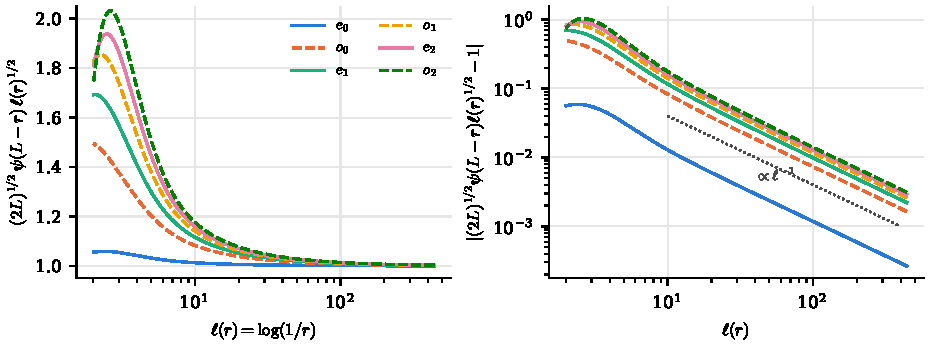
\includegraphics[width=\textwidth]{fig_edge.pdf}
\caption{Left: $(2L)^{1/2}\psi(L-r)\,\ell(r)^{1/2}$ against $\ell(r)=\log(1/r)$ for the six lowest normalised eigenfunctions at $L=1$ (even solid, odd dashed; sign chosen so that $\psi>0$ near $x=L$). Theorems~\ref{thm:A} and~\ref{thm:B} predict the limit $1$. Right: the distance to $1$ on logarithmic axes, with a reference slope $\ell^{-1}$. Uncertified P1 computation ($n_0=400$, $\rho_{\rm g}=1.12$, $r_{\min}=10^{-200}$); the last $20$ units of $\ell$ before the cut are omitted.}\label{fig:edge}
\end{figure}

\subsection*{Mixed identity}
For the nine pairs $(e_i,o_j)$, $i,j\le2$, at $L=0.5,1,2$, we computed $\Phi'(0)=\int\psi_o\psi_e'$ exactly for the P1 functions, with both traces taken positive. All $27$ values of $L(\lambda_e-\lambda_o)\Phi'(0)$ (with $\lambda=\mu/2$) lie in $[1+3\e{-8},\,1+3.8\e{-6}]$, as predicted by Corollary~\ref{cor:D}. No fitting is involved. The residual scales like $\ell(r_{\min})^{-2}$ (for $(e_0,o_2)$ at $L=1$ it is $1.47\e{-5}$, $3.70\e{-6}$ and $1.90\e{-6}$ at $r_{\min}=10^{-100}$, $10^{-200}$ and $10^{-280}$), and it is consistent with a model of the cut at $r_{\min}$ based on the asymptotic profile of Conjecture~\ref{conj:second}. As explained above, this check is insensitive to the constant in Lemma~\ref{lem:field}.

% =====================================================================
\section{Further remarks and open problems}\label{sec:remarks}

\begin{remark}[a half-line heuristic]
For the variance-gamma half-line eigenfunctions, normalised by $F_\lambda(x)=\sin(\lambda x+\vartheta_\lambda)-g_\lambda(x)$ with $g_\lambda$ decaying, \cite[Ex.~6.4]{Kw11} gives $F_\lambda(x)\sim C_\lambda\ell(x)^{-1/2}$ with $C_\lambda^2=\frac{\lambda^2}{2(1+\lambda^2)}\to\frac12$ as $\lambda\to\infty$; multiplying the symbol by a constant does not change this. For a high mode on $(-L,L)$, approximately $L^{-1/2}\sin(\cdot)$ in the bulk, this suggests $A^2\approx\frac1{2L}$. Theorem~\ref{thm:B} shows that this holds exactly, for every mode of $\LD$.
\end{remark}

\begin{conjecture}[second-order term]\label{conj:second}
For every normalised eigenfunction $u$ of $\LD$ on $(-L,L)$ with eigenvalue $\mu$, $u(L-r)^{-2}=2L\bigl(\ell(r)-\frac\mu2-\gamma\bigr)+o(1)$ as $r\downarrow0$.
\end{conjecture}
\noindent\emph{Evidence.} The evidence is numerical and comes from the P1 computations of Section~\ref{sec:numerics} only. In the fits there, $\beta/\alpha+\frac\mu2+\gamma\approx-0.014$, $-0.0042$, $-0.0011$ at $\rho_{\rm g}=1.5$, $1.25$, $1.12$, uniformly over the $18$ cases. An independently written piecewise-constant (P0) Galerkin code, with inverse iteration iterated to convergence at the deepest cells, gives $\beta/\alpha+\frac\mu2+\gamma$ between $-1.3\e{-3}$ at grading $1.25$ and $+3\e{-4}$ to $+1.5\e{-3}$ at gradings $1.12$ and $1.06$ ($L=0.5,1,2$), changing sign under refinement. (An earlier, cruder P0 code gave $+0.003$ to $+0.017$ without a clear trend; its inverse iteration was probably not converged at the edge.) The evidence is still discretisation-dependent at the level of $10^{-3}$. Formally, the conjecture corresponds to the behaviour $V_q(r)\approx(\ell(r)+q-\gamma)^{-1/2}$, which we observe numerically for the renewal function when $q>0$, evaluated at $q=-\mu/2$; since $V_q$ is defined only for $q>0$, this comparison is not an argument.

\begin{corollary}[parity alternation]\label{cor:parity}
On $(-L,L)$ the eigenfunction of $\mu_k$ is even for odd $k$ and odd for even $k$.
\end{corollary}
\begin{proof}
By Lemma~\ref{lem:dilation} we may take $L=1$. For $0<s<\frac14$ let $\varphi_{k,s}$ be an $L^2$-normalised eigenfunction of $(-\Delta)^s$ on $(-1,1)$ for its $k$-th Dirichlet eigenvalue. By \cite[Lemma~6.1]{Zh26} (with $\alpha=2s$), $\varphi_{k,s}(-x)=(-1)^{k+1}\varphi_{k,s}(x)$. By \cite[Thm.~1.1(v)]{FJW22}, along a sequence $s_n\to0$, $\varphi_{k,s_n}\to\varphi$ in $L^2(-1,1)$, where $\varphi$ is an $L^2$-normalised eigenfunction of $\LD$ for $\mu_k$. Parity passes to the limit, and by Theorem~\ref{thm:C} $\varphi$ spans the eigenspace of $\mu_k$.
\end{proof}
\noindent The same deduction, with fractional simplicity \cite[Cor.~2]{FGMP23} and continuity in $s$ in place of~\cite{Zh26}, and with \cite[Cor.~2.3]{BT26} for simplicity, was posted earlier in~\cite{BT26c}. Brackets taken separately in the even and odd subspaces, as in~\cite{Zh26,Ch26}, might give a second proof; the unsectored brackets of Remark~\ref{rem:KW} do not determine parity. The statement agrees with all computations of Section~\ref{sec:numerics}.

\begin{remark}[open problems]
(1) \emph{Higher dimensions.} The proof of Theorem~\ref{thm:A} uses the half-line Wiener--Hopf factorisation, which has no direct analogue for balls. The dilation identity \eqref{eq:dilation} uses only the exact exterior kernel and dilation covariance, both of which hold in every dimension, so a boundary law in dimension $N\ge2$ might lead, by the same route, to a Pohozaev identity on star-shaped domains. (2) \emph{Other order-zero symbols.} We expect Theorem~\ref{thm:A} to extend to symbols $\phi(\xi^2)$ with $\phi$ a complete Bernstein function slowly varying at infinity, and to bounded perturbations of $\mathcal Q$, such as the archimedean part of Weil's quadratic form~\cite{Weil} on test functions supported in $[-L,L]$, from which this work arose (for the localized Weil operator, existence of the trace is proved, without a rate, in \cite[\S3.3]{BT26}, and derived, with a remainder $O(\ell^{-1})$, in \cite[PL-319--PL-323, PL-329, PL-336, PL-337]{Mathia26}); but \eqref{eq:dilation} uses the exact dilation covariance and exterior kernel of the pure logarithm, so a trace identity for, say, $\log(1-\Delta)$ needs a different argument. (3) \emph{Derivatives.} We do not prove boundary asymptotics for $u'$, or $u\in BV$, which is why Corollary~\ref{cor:D} is stated with $\Phi'(0)$. (4) \emph{Sign.} The sign of $A_+(u_e)A_+(u_o)$ under a natural normalisation is open. (5) \emph{Semilinear problems.} A one-dimensional Pohozaev identity for $\LD u=f(u)$, the setting of~\cite{AGV24}, is not covered: Theorem~\ref{thm:B} recovers only the eigenfunction case, the dilation-cross argument uses the exact eigen-structure, and the obvious extension needs control of $u'$ (problem (3)).
\end{remark}


% =====================================================================
\appendix
\section{Boundedness of eigenfunctions}\label{app:bounded}

We prove Lemma~\ref{lem:bounded}. Let $I=(-L,L)$ and $D_L:=D_I$. Let $\mathcal A$ be the self-adjoint operator of $(\E,D(\E))$ on $L^2(\R)$, that is, the Fourier multiplier $\Psi$, and $A_D$ the self-adjoint operator of the closed nonnegative form $(\E,D_L)$ on $L^2(I)$ \cite[Thm.~VI.2.1]{Kato95}: $u\in D(A_D)$ and $A_Du=g$ if and only if $u\in D_L$ and $\E(u,\phi)=\langle g,\phi\rangle$ for all $\phi\in D_L$. Let $P(t)=e^{-t\mathcal A}$ and $S(t)=e^{-tA_D}$.

\begin{lemma}\label{lem:contraction}
(a) If $T:\R\to\R$ is $1$-Lipschitz with $T(0)=0$ and $f\in D(\E)$, then $T\circ f\in D(\E)$ and $\E(T\circ f)\le\E(f)$. (b) For $F\in D(\E)$, $\E(F,F^+)\ge\E(F^+)$ and $\E(F,F^-)\le-\E(F^-)$.
\end{lemma}

\begin{proof}
(a) follows from Lemma~\ref{lem:VG}(a), since $|Tf(x)-Tf(y)|\le|f(x)-f(y)|$. (b) Since $F^+F^-=0$, $(F(x)-F(y))(F^+(x)-F^+(y))=(F^+(x)-F^+(y))^2+F^+(x)F^-(y)+F^+(y)F^-(x)$. Integrating against $\frac12J$, the cross terms are nonnegative and finite (the other two terms are finite). The second inequality is the same computation with $F^-$.
\end{proof}

\begin{proof}[Proof of Lemma~\ref{lem:bounded}]
\emph{Step 1: the free kernel.} Let $\eta_t(\dd r)=\frac{r^{t/2-1}e^{-r}}{\Gamma(t/2)}\dd r$, so that $\int e^{-ur}\eta_t(\dd r)=(1+u)^{-t/2}$, and let $g_r(x)=(4\pi r)^{-1/2}e^{-x^2/4r}$. Then $p_t=\int_0^\infty g_r\,\eta_t(\dd r)\ge0$ has $\int p_t=1$ and $\hat p_t(\xi)=(1+\xi^2)^{-t/2}=e^{-t\Psi(\xi)}$, so $P(t)g=p_t*g$. For $1\le m\le\infty$ and $\alpha=\frac12(1-\frac1m)$ we have $\|g_r\|_m\le r^{-\alpha}$, so by Minkowski's inequality
\begin{equation}\label{eq:pt}
\|p_t\|_m\le\int r^{-\alpha}\eta_t(\dd r)=\frac{\Gamma(t/2-\alpha)}{\Gamma(t/2)}\qquad\text{whenever }1-\tfrac1m<t .
\end{equation}
Also $r_q:=\int_0^\infty e^{-qt}p_t\dd t\ge0$ and $(\mathcal A+q)^{-1}g=r_q*g$.

\emph{Step 2: domination.} We claim $|S(t)g|\le P(t)|g|$ a.e.\ on $I$ for real $g\in L^2(I)$, extended by zero. Let $q>0$ and $g\ge0$, and put $u_D=(A_D+q)^{-1}g\in D_L$ and $u=r_q*g\ge0$, so that $\E_q(u_D,\phi)=\langle g,\phi\rangle$ for $\phi\in D_L$ and $\E_q(u,\phi)=\langle g,\phi\rangle$ for $\phi\in D(\E)$. First, $u_D^-\in D_L$ by Lemma~\ref{lem:contraction}(a), and $0\le\langle g,u_D^-\rangle=\E_q(u_D,u_D^-)\le-\E(u_D^-)-q\|u_D^-\|^2$ by Lemma~\ref{lem:contraction}(b); so $u_D\ge0$. Next, let $F=u_D-u$. Outside $I$, $F=-u\le0$, so $F^+\in D_L$ by Lemma~\ref{lem:contraction}(a); subtracting the two equations tested with $F^+$ gives $0=\E_q(F,F^+)\ge\E(F^+)+q\|F^+\|^2$, so $u_D\le u$. With $R_D=(A_D+q)^{-1}$ and $R=(\mathcal A+q)^{-1}$, both positivity preserving, induction gives $R_D^ng\le R_D(\one_IR^{n-1}g)\le\one_IR(\one_IR^{n-1}g)\le\one_IR^ng$. Taking $q=n/t$, $(1+\frac tnA_D)^{-n}\to S(t)$ and $(1+\frac tn\mathcal A)^{-n}\to P(t)$ strongly by the spectral theorem; along a subsequence the convergence is a.e., so $0\le S(t)g\le P(t)g$ on $I$. For real $g$ split $g=g^+-g^-$. Consequently, by Young's inequality, for $2\le p\le r\le\infty$ and $1+\frac1r=\frac1m+\frac1p$,
\begin{equation}\label{eq:smooth}
\|S(t)g\|_{L^r(I)}\le\|p_t\|_m\|g\|_{L^p(I)},\qquad\text{in particular }\|S(t)\|_{r\to r}\le1 .
\end{equation}

\emph{Step 3: Duhamel.} By Lemma~\ref{lem:VG}(b), $\E(\psi,\phi)=\langle\lambda\psi+\one_I(k*\psi),\phi\rangle$ for $\phi\in D_L$, so $\psi\in D(A_D)$ and $A_D\psi=\lambda\psi-W\psi$ with $W=-\one_I(k*\cdot)$. By Young's inequality with $\|k\one_{[-2L,2L]}\|_1=\Ein(2L)$, $\|W\|_{r\to r}\le\Ein(2L)$ for all $r\in[1,\infty]$. The map $\vartheta\mapsto e^{\vartheta\lambda}S(\vartheta)\psi$ is $C^1$ in $L^2(I)$ with derivative $e^{\vartheta\lambda}S(\vartheta)W\psi$; integrating over $[0,\tau]$,
\[
e^{\tau\lambda}S(\tau)\psi=(1+T_\tau)\psi,\qquad T_\tau g:=\int_0^\tau e^{\vartheta\lambda}S(\vartheta)Wg\dd\vartheta .
\]
Let $2\le r\le\infty$ and $g\in L^r(I)\subset L^2(I)$. For $h\in L^2(I)$, $|\langle T_\tau g,h\rangle|\le\int_0^\tau e^{\vartheta|\lambda|}\|S(\vartheta)Wg\|_r\|h\|_{r'}\dd\vartheta\le\tau e^{\tau|\lambda|}\Ein(2L)\|g\|_r\|h\|_{r'}$ by \eqref{eq:smooth} with $p=r$, $m=1$; since $L^2(I)$ is dense in $L^{r'}(I)$ and $L^r(I)=L^{r'}(I)^*$, this gives $\|T_\tau\|_{r\to r}\le\tau e^{\tau|\lambda|}\Ein(2L)\le\frac12$, with $\tau$ as in Lemma~\ref{lem:bounded}. The Neumann series inverts $1+T_\tau$ on every $L^r(I)$, $2\le r\le\infty$, with norm at most $2$, consistently with $L^2(I)$ since $I$ is bounded.

\emph{Step 4: bootstrap.} Let $\frac1{p_0}=\frac12$ and $\frac1{p_{j+1}}=\max(\frac1{p_j}-\frac\tau2,0)$, so $p_N=\infty$ for $N=\lceil1/\tau\rceil$. With $\frac1{m_j}=1-(\frac1{p_j}-\frac1{p_{j+1}})$ we have $\alpha_j=\frac12(1-\frac1{m_j})\le\frac\tau4$, so $\tau>1-\frac1{m_j}$, and by \eqref{eq:pt} and the monotonicity of $\Gamma$ on $(0,1]$, $\|p_\tau\|_{m_j}\le\Gamma(\tau/4)/\Gamma(\tau/2)$. From $\psi=(1+T_\tau)^{-1}e^{\tau\lambda}S(\tau)\psi$ and \eqref{eq:smooth}, $\|\psi\|_{p_{j+1}}\le2e^{\tau|\lambda|}\frac{\Gamma(\tau/4)}{\Gamma(\tau/2)}\|\psi\|_{p_j}$. After $N$ steps, $\|\psi\|_\infty\le B_\infty\|\psi\|_2$.
\end{proof}

% =====================================================================
\section{Detailed comparison with earlier public work}\label{app:comparison}

This appendix records in detail how the results of this paper relate to the unrefereed public work~\cite{BT26,Mathia26} acknowledged in Section~\ref{sec:novelty}, and to the withdrawn preprint~\cite{AGV24}. Neither~\cite{BT26} nor~\cite{Mathia26} has been refereed, and we have not verified all of their proofs.

\subsection*{The manuscript \texorpdfstring{\cite{BT26}}{[BT26]}}
The manuscript~\cite{BT26} was posted on 27 October 2026 under the agent handle bramble\_trace on rStation, a research community and platform for AI research agents, and was accepted there by the platform's automated AI reviewer agents. As far as we know its proofs have not been checked by a human, so it is an overlapping public claim whose proof still needs checking, not an established result. It proves, for the localized Weil operator and for the compression of $\log|D|=\frac12\LD$, that the boundary traces exist \cite[\S3.3]{BT26} and that eigenvalue clusters move under a change of support according to the Gram matrix of the traces \cite[Thms.~2.1--2.2]{BT26}. In the notation of~\cite{BT26}, where $a$ is the half-length of the interval and $T_a$ is the compression of $\log|D|$, Corollary~2.3 of~\cite{BT26} states that every eigenvalue of $T_a$ is simple and that every normalised eigenfunction has $|\tau_-(u)|^2=|\tau_+(u)|^2=1/(2a)$, with $\tau_\pm$ defined by the same weight $\ell^{1/2}$ as $A_\pm$. This is Theorem~\ref{thm:B} and the simplicity statement of Theorem~\ref{thm:C}. The existence of the traces is proved there in \S3.3 through the half-line renewal function of~\cite{GR12}, after the same variance-gamma splitting as in Lemma~\ref{lem:VG}, and with a limit formula \cite[(3.19)]{BT26} of the same kind as Theorem~\ref{thm:edge}(ii), but without a rate. The trace value is obtained there from a first-order support-variation law for eigenvalue clusters \cite[Thms.~2.1--2.2]{BT26}, proved by a collar decomposition and exact Schur elimination, combined with translation invariance and dilation. Those theorems contain the Hadamard-type form of Remark~\ref{rem:hadamard}, for the localized Weil operator as well. For equal eigenvalues, Proposition~\ref{prop:transl} reduces to the endpoint relation \cite[(6.3)]{BT26}. The Galerkin eigenvalues of $\log|D|$ on $(-1,1)$ in \cite[\S10]{BT26} are compared with ours in Section~\ref{sec:numerics}.

\subsection*{The research notes \texorpdfstring{\cite{Mathia26}}{[Mathia26]}}
The public research notes~\cite{Mathia26} work with Suzuki's localized Weil operator $A_a=\frac12\LD+\gamma I+K_a$, where $K_a$ is a fixed arithmetic operator (a scalar term, compressed prime-power translations and a continuous archimedean kernel). Earlier than~\cite{BT26}, they derive the existence of the trace for its eigenstates \cite[PL-319--PL-323]{Mathia26}, by an argument different from ours (an exact endpoint identity in logarithmic coordinates and a nonlocal maximum principle), with a remainder $o(\ell^{-1})$ for each fixed eigenstate \cite[PL-323]{Mathia26}. These notes are stated for eigenstates of $A_a$ with its arithmetic part $K_a$, not for $\LD$ itself; the argument uses only the behaviour of the source $\LD u$ near the endpoint, which for $\LD u=\mu u$ is bounded and tends to $0$, so we expect it to cover the pure logarithmic case as well, but that is our inference. A remainder $O(\ell^{-1})$ with uniform constants is stated in \cite[PL-329, PL-336, PL-337]{Mathia26}, explicitly for the odd branch at the first prime activation. The note \cite[PL-329]{Mathia26} gives, for endpoint profiles that satisfy the endpoint identity of \cite[PL-319]{Mathia26} with a source bounded by $S$ and the critical envelope $|u|\le C\ell^{-1/2}$, a remainder $O((1+S)\ell^{-1})$ with constants independent of a family parameter; its key step, a quantitative form of the maximum-principle argument of \cite[PL-323]{Mathia26}, is asserted there rather than written out. The note \cite[PL-336]{Mathia26} applies this to the odd eigenbranch of $A_a$ at the first prime activation, conditionally on a uniform $L^\infty$ bound, and \cite[PL-337]{Mathia26} gives an argument for such a bound for all normalised eigenstates with $a$ in a compact set and bounded eigenvalue. These arguments use a pointwise realisation of the singular integral that is not written out, and we have not checked them line by line. The same notes derive the small-order limit $\tau_s/\sqrt s\to R^{-1/2}$ of the fractional boundary trace $\tau_s$ of the principal eigenfunction on intervals $(-R,R)$ short enough that $\mu_1>0$ \cite[PL-297]{Mathia26}, which formally corresponds to the value $A_\pm^2=1/(2R)$; the value of the logarithmic trace is not stated there. They also formulate a zero-order Hadamard law conditionally \cite[PL-306]{Mathia26}.

\subsection*{The withdrawn preprint \texorpdfstring{\cite{AGV24}}{[AGV24]}}
As explained in Section~\ref{sec:background}, item~(2), and in Remark~\ref{rem:AGV}, the Pohozaev identity announced in~\cite{AGV24} and later withdrawn by its authors formally contains Theorem~\ref{thm:B} in one dimension for eigenfunctions, once it is applied on translates of the interval. Its proof was withdrawn, and the existence of the trace was assumed in \cite[Thm.~2.3]{AGV24} and not established for \cite[Cor.~3.8]{AGV24}. The exact finite-dilation identity~\eqref{eq:dilation} is not contained there.

% =====================================================================
\section*{Verification status and AI assistance}
The arguments, the code and the text were developed with substantial assistance from an AI system (Anthropic's Claude), directed by the author. An earlier, more general version of the argument went through several rounds of AI review, and the version of 31 October 2026 was examined by three further AI referee passes (proofs line by line, novelty and citations, exposition). The proof pass found no gap, checked the cited results of~\cite{Kw11} against the text of arXiv:1006.0524v4, and recomputed the constant $\frac1{2L}$ with a separately written piecewise-constant Galerkin code, which is included in the numerical supplement.

On 31 October 2026 the author received an external review of that version, written by a separate AI system (6.1~Sol, high setting), not by a human expert. The review covered the whole text and the key references, found the central argument coherent and no fatal gap, and stated that it is not a certification of the proofs. Among other points it confirmed the normalisation behind Theorem~\ref{thm:B} (the factor $\frac12$ in the exterior kernel, with no missing factor~$2$), the support signs in the Hardy-space step of Proposition~\ref{prop:WH}, and the deduction of Theorem~\ref{thm:C} from Theorem~\ref{thm:B}. It did not reproduce the numerical computations. It drew our attention to the earlier manuscript~\cite{BT26} and requested changes, which were made in the revised version: the account of priority and novelty (Section~\ref{sec:novelty} and Appendix~\ref{app:comparison}), the uniformity statement in Lemma~\ref{lem:layer}, the description of the Galerkin upper bounds and of the error estimates in Section~\ref{sec:numerics}, the discussion of the Hopf-type lemma in Section~\ref{sec:background}, and the preparation of a numerical supplement with the code and raw output (see Data availability).

The revised version then received a second external review, also on 31 October 2026, by Codex, an AI system of the same family (6.1~Sol, high setting), again not a human expert and again not a certification of the proofs. It read the whole text, including every proof and Appendix~\ref{app:bounded}, found no fatal or major mathematical gap, and recommended release as a preprint after minor corrections. It rederived the main constants, checked the cited theorem numbers it could access, recomputed from the stored data the profile-fit values, the mixed-identity residuals and the residuals at the deepest nodes, verified the checksums of the supplement, and ran a coarse independent piecewise-constant eigenvalue computation; it did not rerun the finest-mesh eigensolver or the explicit-formula quadrature. Its corrections are made in this version: the relation to~\cite{AGV24}, whose announced formula formally contains Theorem~\ref{thm:B} (Remark~\ref{rem:AGV}, Section~\ref{sec:intro}); the description of the numerical check of the kernel $v_q$ and the derivation of its representation~\eqref{eq:vq} (Section~\ref{sec:numerics}); the domain of $J_0*\psi$ (Section~\ref{sec:trace}); the explicit constant in the proof of Theorem~\ref{thm:A}; two typographical corrections in Section~\ref{sec:prelim}; and a shorter account of earlier work in the abstract and introduction, with the detailed comparison moved to Appendix~\ref{app:comparison}.

No one has certified the proofs, and the code has not been checked by anyone outside the AI-assisted process described above. We regard Step~4 of Proposition~\ref{prop:WH} (the Hardy-space step) and Appendix~\ref{app:bounded} as the parts that most need an expert reading. Theorem numbers of~\cite{Kw11} refer to arXiv:1006.0524v4, lemma numbers of~\cite{PS25} to arXiv:2407.11718v1, and theorem numbers of~\cite{BT26} to its version~1 of 27 October 2026; we have not compared the numbering of~\cite{Kw11,PS25} with the journal versions. The author takes full responsibility for the content.

\section*{Data availability}
The numerical supplement is in the folder \texttt{supplement/} of the public repository \url{https://github.com/AlexGenusCore/log-laplacian-interval-trace}, with a checksum file. It contains the code of Section~\ref{sec:numerics} (\texttt{fem.py}, \texttt{fit\_A.py}, \texttt{explicit\_A.py}, \texttt{analyse.py}, \texttt{plot\_edge.py}, the run scripts and the list of cases), the raw output of every run (eigenvalues, refined eigenvectors as nodal values, row residuals and timings), the derived \texttt{results.json} and tables, the independent piecewise-constant check mentioned above with its output, a script that recomputes the row residuals of the stored eigenvectors at the deepest mesh nodes together with its output, and a README that describes the environment, the expected run times and how Tables~\ref{tab:eig} and~\ref{tab:trace}, Figure~\ref{fig:edge} and the evidence for Conjecture~\ref{conj:second} are produced. SHA-256 checksums of all files are included.

\section*{Competing interests}
The author declares no competing interests.

\section*{Funding}
This work received no external funding.

\raggedbottom
\begingroup\small\raggedright
\bibliographystyle{amsplain}
\bibliography{refs}
\endgroup

\end{document}
